\documentclass[xcolor=table,ps]{beamer}
\usepackage{listings}
\usepackage[english]{babel}         
\usepackage[utf8x]{inputenc}      
\usepackage{multirow}
\usepackage{colortbl}
\usepackage{ltablex}
\usepackage{courier}
\usepackage{subfigure}
\usepackage{wrapfig}
\usepackage{ragged2e}
\usepackage{setspace}
\usepackage{caption}
\usepackage{adjustbox}
\usepackage[justification=centering, labelformat=empty]{caption}
\captionsetup[figure]{font={stretch=0.5}}
\usepackage{cancel}
\usepackage{adjustbox}
\usepackage[labelformat=empty]{caption}
\usepackage{graphicx}

% \usepackage{subfig}
%%%%%%%%%%%%%%%%%%%%%%%%%%%%%%%%%%%%%%%%%%%%%%%

%\usetheme{Boadilla}
\usetheme{Madrid}
\setbeamertemplate{navigation symbols}{}
\setbeamertemplate{footline}[frame number]

\setbeamercolor*{bibliography entry note}{fg=black}
\setbeamertemplate{bibliography item}{\insertbiblabel}

\definecolor{gray_c}{rgb}{0.0,0.0,0.5}
\definecolor{gray0}{gray}{0.6}
\definecolor{gray1}{gray}{0.8}
\definecolor{gray2}{gray}{0.85}
\definecolor{gray3}{gray}{0.7}

\definecolor{col0}{rgb}{0.88,1,1}

\newcolumntype{g}{>{\columncolor{gray1}}c}
\newcolumntype{t}{>{\columncolor{gray0}}c}
\usecolortheme[named=gray_c]{structure}
\definecolor{apceleste}{rgb}{0.0,0.0,0.99}

%%%%%%%%%%%%%%%%%%%%%%%%%%%%%%%%%%%%%%%%%%%%%%%%%%%%%%%%%%%%%%%%%%%
%% Personal Information
%%%%%%%%%%%%%%%%%%%%%%%%%%%%%%%%%%%%%%%%%%%%%%%%%%%%%%%%%%%%%%%%%%%
\title[FFT Architecture via Folding Transformation]{\textbf{VLSI Implementation of a Pipelined 128 points 4-Parallel radix-$\mathbf{2^3}$ FFT Architecture via Folding Transformation}} 
    
    
\author[]{
James J. W. Kunst  {\tt\small jjwk89@gmail.com}\\		
Kevin H. Viglianco	{\tt\small kevinviglianco@gmail.com}\\	 
Daniel R. Garcia	{\tt\small dani6rg@gmail.com}
%\vspace{0.5cm}
%Dr. Keshab K. Parhi	\\
%Dr. Ariel L. Pola	\\
}

\date{\today} % (optional)

\titlegraphic{\vspace{0.3cm}
\includegraphics[width=0.2\paperwidth]{./logo_ff.eps}}

\makeatletter
\@addtoreset{subfigure}{framenumber}% subfigure counter resets every frame
\makeatother

%%%%% Para código fuente y reportes
\usepackage{listings}
\definecolor{mygreen}{rgb}{0,0.6,0}
\definecolor{mygray}{rgb}{0.5,0.5,0.5}
\definecolor{mymauve}{rgb}{0.58,0,0.82}
\definecolor{mygrayV}{rgb}{0.8,0.8,0.8}

\lstset{
  backgroundcolor=\color{mygrayV},
  basicstyle=\tiny,%\scriptsize,%\footnotesize, 
  breakatwhitespace=false,
  breaklines=true,
  captionpos=b,
  commentstyle=\color{mygreen},
  deletekeywords={...},
  escapeinside={\%*}{*)},
  extendedchars=true,
  frame=single,
  keepspaces=true,
  keywordstyle=\color{blue},
  language=Verilog,
  morekeywords={*,...},
  numbers=left,
  numbersep=3pt,
  numberstyle=\tiny\color{mygray},
  rulecolor=\color{black},
  showspaces=false,
  showstringspaces=false,
  showtabs=false,
  stepnumber=1,
  stringstyle=\color{mymauve},
  tabsize=2,
  %title=\lstname
  framerule=0pt,
  aboveskip=0pt,
  framextopmargin=0pt,
  framexbottommargin=0pt,
  %framexleftmargin=3pt,
  framesep=0.1pt,
  rulesep=.4pt,
  rulesepcolor=\color{blue},
  numberfirstline = true,
}

\begin{document}

%%%%%%%%%%%%%%%%%%%%%%%%%%%%%%%%%%%%%%%%%%%%%%%%%%%%%%%%%%%%%%%%%%%
%% Title Frame
%%%%%%%%%%%%%%%%%%%%%%%%%%%%%%%%%%%%%%%%%%%%%%%%%%%%%%%%%%%%%%%%%%%
\begin{frame}
%  \vspace{1.cm}
  \titlepage
\end{frame}

%%%%%%%%%%%%%%%%%%%%%%%%%%%%%%%%%%%%%%%%%%%%%%%%%%%%%%%%%%%%%%%%%%%
%% Logo Lower-Left
%%%%%%%%%%%%%%%%%%%%%%%%%%%%%%%%%%%%%%%%%%%%%%%%%%%%%%%%%%%%%%%%%%%

\usebackgroundtemplate{
\setlength{\unitlength}{1mm}
\begin{picture}(1,1)
 \linethickness{0.5mm}
  \put(0,-94){
\includegraphics[height=0.4cm]{./logo_ff.eps}}
\end{picture}
}

\begin{frame} 
  \frametitle{\textbf{Tabla de Contenidos}}
  \tableofcontents
  % \mframetitle{Outline}
\end{frame}

%%%%%%%%%%%%%%%%%%%%%%%%%%%%%%%%%%%%%%%%%%%%%%%%%%%%%%%%%%%%%%%%%%%
%% Frames
%%%%%%%%%%%%%%%%%%%%%%%%%%%%%%%%%%%%%%%%%%%%%%%%%%%%%%%%%%%%%%%%%%%

%%%%%%%%%%%%%%%%%%%%%%%%%%%%%%%%%%%%%%%%%%%%%%%%%%%%%%%%%%%%%%%%%%% 
%% Introduccion y desarrollo del algoritmo
%%%%%%%%%%%%%%%%%%%%%%%%%%%%%%%%%%%%%%%%%%%%%%%%%%%%%%%%%%%%%%%%%%%


\section{Introduction}
\begin{frame}
  \frametitle{\textbf{Table of Contents}}
  \begin{center}
    {\vspace{-1.5cm}\Large \textbf{Section \thesection}\vspace{0.5cm}}
    \begin{beamercolorbox}[
      sep=8pt,center]{part title}
      \usebeamerfont{part title}
      \textbf{\insertsection}
    \end{beamercolorbox}
  \end{center}
\end{frame}


\begin{frame}
	\frametitle{\textbf{Introduction}}
	\framesubtitle{\secname : \subsecname}
	\begin{block}{\centering \textbf{Objetives}}
		\begin{itemize} \justifying\footnotesize
  			\item Design and implement a 4-parallel pipelined architecture for the Complex Fast Fourier Transform (CFFT) based on the radix-$2^3$ algorithm with 128 points 	using folding transformation and register minimization techniques based on ... .
   			\item Frecuency of implementation: 500MHz. 
  			\item Optimization with CSD\footnote{Canonic Signed Digit} multipliers.
  			\item Test the design with a mixture of two sinusoids using MATLAB.
  			\item Generate power-area-timing report with different
			optimizations. 			
  		\end{itemize}
    \end{block}
\end{frame}



\begin{frame}
	\frametitle{\textbf{Introduction}}
	\framesubtitle{\secname : \subsecname}
	\begin{block}{\centering \textbf{Workflow}}
		\begin{enumerate} \justifying\footnotesize
			\item Obtain the equations that correspond to Butterfly structure of radix-$2^3$ FFT for 8 points.
			\item Apply this idea to design a 2-parallel pipelined architecture radix-$2^3$ 16-points FFT via folding transformation.
			\item Traslate this to a 128-points model.
			\item Elaborate a float-point simulator in Matlab of the 128-points.
			\item Elaborate a synthesizable verilog code HDL and verify the DFT functionality.
			\item Generates power-area-timing report with different optimizations.
		\end{enumerate}
    \end{block}
\end{frame}


\begin{frame}
	\frametitle{\textbf{Introduction}}
    \framesubtitle{\secname : \subsecname}
	\begin{block}{\centering \textbf{Types of pipelined Radix-2 FFT architectures}}
		\begin{enumerate} \justifying\footnotesize
  			\item Feedfoward Multi-Path Delay Commutator (MDC).
  			\item Single-Path Delay Feedback architectures (SDF).
  		\end{enumerate}
		\begin{itemize} \justifying\footnotesize
  			\item Both butterflies and multipliers are in 50\% utilization ... .
  			\item The SDF use registers more efficiently.
  			\item We will focus on the feedfoward MDC asrchitecture.
  		\end{itemize}
    \end{block}

    \vspace{-0.2cm}
    \begin{figure}[!t] \centering
    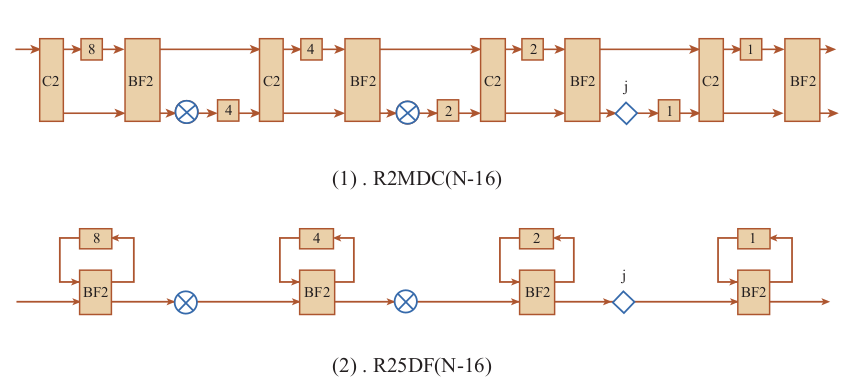
\includegraphics[width=0.70\paperwidth]{./image/types_FFT.png}
    \end{figure}
\end{frame}
   % Introducción 
\section{The Radix-$2^3$ FFT  Algorithm}
\begin{frame}
  \frametitle{\textbf{Table of Contents}}
  \begin{center}
    {\vspace{-1.5cm}\Large \textbf{Section \thesection}\vspace{0.5cm}}
    \begin{beamercolorbox}[
      sep=8pt,center]{part title}
      \usebeamerfont{part title}
      \textbf{\insertsection}
    \end{beamercolorbox}
  \end{center}
\end{frame}

\begin{frame}
	\frametitle{\textbf{The Radix-$2^3$ FFT  Algorithm}}
	\framesubtitle{\secname : \subsecname}
	\begin{block}{\centering \textbf{\textit{N}-point DFT of an input sequence $x[n]$}}
		\begin{equation}
			X[k] = \sum_{n=0}^{N-1} x[n] \cdot W_N^{nk}, \quad k=0,1,...,N-1 \qquad
		\end{equation}
		where $W_N^{nk} = e^{-j\frac{2\pi}{N} nk}$. 
	\end{block}
	
	\begin{block}{\centering}
		\begin{itemize}\justifying\footnotesize
			\item Direct computation of the DFT is inefficient because it does not exploit the properties of:
			\begin{enumerate}
				\item Symmetry: $ W_N^{k+N/2} = -W_N^k$
				\item Periodicity:  $W_N^{k+N} = W_N^k$
			\end{enumerate}
			\item The FFT based on Cooley-Tukey algorithm reduce the number of operations from $O(N^2)$ for the DFT to $O(Nlog_2N)$ for the FFT.
		\end{itemize}	
	\end{block}
\end{frame}


\begin{frame}
  	\frametitle{\textbf{The Radix-$2^3$ FFT  Algorithm}}
	\framesubtitle{\secname : \subsecname}
	\begin{block}{\centering \textbf{\textit{Divide and Conquer} approach}}
		\begin{itemize} \justifying\footnotesize		
			\item We can calculate the DFT in series of $s=log_\rho N$ stages, where $\rho$ is the base of the \textit{radix}. 
			\item This is based on the decomposition of an N point DFT into successively smaller DFTs.
			\item  In our case, the numeber of stages is:
		 	\begin{equation}
		 			s = log_2 (128) = 7 
		 	\end{equation}
		\end{itemize}		
	\end{block}

	\begin{block}{\centering \textbf{Methods to design FFT algorithms}}
		\begin{enumerate} \justifying\footnotesize
			\item \textbf{Decimation In Time (DIT):} Splitting successively data sequence $x[n]$ by a factor of 2. 					
			\item \textbf{Decimation In Frcuency (DIF):} Splitting successively the data sequence $X[k]$ by a factor of 2. 
		\end{enumerate}											
  	\end{block}
\end{frame}

\begin{frame}
  	\frametitle{\textbf{The Radix-$2^3$ FFT  Algorithm}}
	\framesubtitle{\secname : \subsecname}
	\begin{block}{\centering \textbf{DIT and DIF Butterflies}}
		The difference is the instant in which the multiplication by $W_N^\phi$ is accomplished. 
	\end{block}    	
    	\vspace{-0.2cm}
    	\begin{figure}[h!] \centering
    		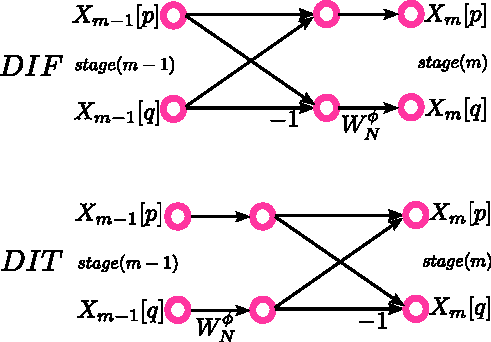
\includegraphics[width=0.45\paperwidth]{./image/DifDit.pdf}
    	\end{figure}
\end{frame}

\begin{frame}
  	\frametitle{\textbf{The Radix-$2^3$ FFT  Algorithm}}
	\framesubtitle{\secname : \subsecname}
	\begin{block}{\centering \textbf{Order of samples in DIT and DIF}}
		\begin{itemize}\justifying\footnotesize
			\item  The input samples in FFT algorithms DIF are organized in natural order but its output has not in order.
			\item The opposite is for DIT.
		\end{itemize}
	\end{block}    	
    \begin{figure}[h!] \centering
    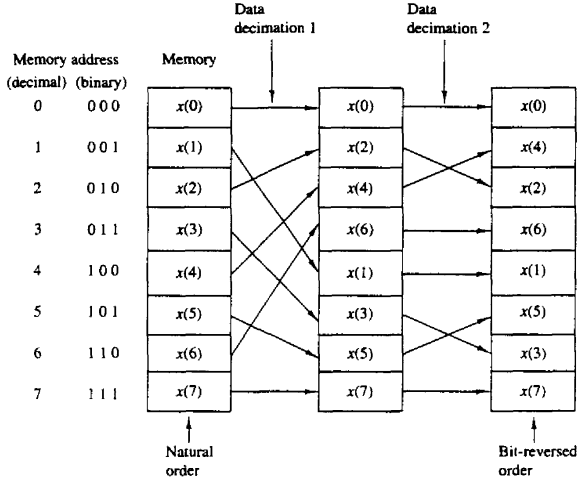
\includegraphics[width=0.4\paperwidth]{./image/dif_order.png}
    	\caption{\footnotesize Order of intpus and outputs for DIF FFT.} % Añadir referencia
    \end{figure}
\end{frame}



\begin{frame}
  	\frametitle{\textbf{The Radix-$2^3$ FFT  Algorithm}}
	\framesubtitle{\secname : \subsecname}
	\begin{block}{\centering \textbf{Mathematic expression of radix-8 butterfly element}}
		\vspace{-0.3cm}		 
		 \scalebox{0.55}{
			\label{eqn:radix}		 
		 \parbox{\linewidth}{    		
		\begin{align}			
		C_{8k+0} = \sum_{n=0}^{N/8-1} \bigg\{&[(x_n + x_{n+\frac{N}{2}}) + (x_{n+\frac{N}{4}} + x_{n+\frac{3N}{4}})] + [(x_{n+\frac{N}{8}} + x_{n+\frac{5N}{8}}) + (x_{n+\frac{3N}{8}} + x_{n+\frac{7N}{8}})] \bigg\} W_N^{0n} W_{N/8}^ {nk}     \nonumber \\
		%	
		C_{8k+4} = \sum_{n=0}^{N/8-1} \bigg\{&[(x_n + x_{n+\frac{N}{2}}) + (x_{n+\frac{N}{4}} + x_{n+\frac{3N}{4}})] - [(x_{n+\frac{N}{8}} + x_{n+\frac{5N}{8}}) + (x_{n+\frac{3N}{8}} + x_{n+\frac{7N}{8}})] \bigg\} W_N^{4n} W_{N/8}^ {nk}     \nonumber\\
		%
		C_{8k+2} = \sum_{n=0}^{N/8-1} \bigg\{&[(x_n + x_{n+\frac{N}{2}}) - (x_{n+\frac{N}{4}} + x_{n+\frac{3N}{4}})] -j [(x_{n+\frac{N}{8}} + x_{n+\frac{5N}{8}}) - (x_{n+\frac{3N}{8}} + x_{n+\frac{7N}{8}})] \bigg\} W_N^{2n} W_{N/8}^ {nk}     \nonumber\\
		%
		C_{8k+6} = \sum_{n=0}^{N/8-1} \bigg\{&[(x_n + x_{n+\frac{N}{2}}) - (x_{n+\frac{N}{4}} + x_{n+\frac{3N}{4}})] +j	[(x_{n+\frac{N}{8}} + x_{n+\frac{5N}{8}}) - (x_{n+\frac{3N}{8}} + x_{n+\frac{7N}{8}})] \bigg\} W_N^{6n} W_{N/8}^ {nk}     \nonumber\\
		%
		C_{8k+1} = \sum_{n=0}^{N/8-1} \bigg\{&[(x_n - x_{n+\frac{N}{2}}) -j (x_{n+\frac{N}{4}} - x_{n+\frac{3N}{4}})] + W_N^{N/8} [(x_{n+\frac{N}{8}} - x_{n+\frac{5N}{8}}) -j (x_{n+\frac{3N}{8}} - x_{n+\frac{7N}{8}})] \bigg\} W_N^{n} W_{N/8}^ {nk}     \nonumber\\
		%
		C_{8k+5} = \sum_{n=0}^{N/8-1} \bigg\{&[(x_n - x_{n+\frac{N}{2}}) -j (x_{n+\frac{N}{4}} - x_{n+\frac{3N}{4}})] - W_N^{N/8} [(x_{n+\frac{N}{8}} - x_{n+\frac{5N}{8}}) -j (x_{n+\frac{3N}{8}} - x_{n+\frac{7N}{8}})] \bigg\} W_N^{5n} W_{N/8}^ {nk}    \nonumber\\
		%
		C_{8k+3} = \sum_{n=0}^{N/8-1} \bigg\{&[(x_n - x_{n+\frac{N}{2}}) +j (x_{n+\frac{N}{4}} - x_{n+\frac{3N}{4}})] + W_N^{3N/8} [(x_{n+\frac{N}{8}} - x_{n+\frac{5N}{8}}) +j (x_{n+\frac{3N}{8}} - x_{n+\frac{7N}{8}})] \bigg\} W_N^{3n} W_{N/8}^ {nk}    \nonumber\\
		%
		C_{8k+7} = \sum_{n=0}^{N/8-1} \bigg\{&[(x_n - x_{n+\frac{N}{2}}) +j (x_{n+\frac{N}{4}} + x_{n+\frac{3N}{4}})] - W_N^{3N/8} [(x_{n+\frac{N}{8}} - x_{n+\frac{5N}{8}}) +j (x_{n+\frac{3N}{8}} - x_{n+\frac{7N}{8}})] \bigg\} W_N^{7n} W_{N/8}^ {nk}    \nonumber 	
		\end{align}}}
	\end{block}
    
    
\end{frame}

\begin{frame}
  	\frametitle{\textbf{The Radix-$2^3$ FFT  Algorithm}}
	\framesubtitle{\secname : \subsecname}
	\begin{block}{\centering \textbf{Radix-$2^k$ Implementation}}
		The quantity of rotators of an architecture radix-$2^k$ (with $k>1$) is less than the radix-2.
	\end{block}
    \begin{figure}[h!] \centering
    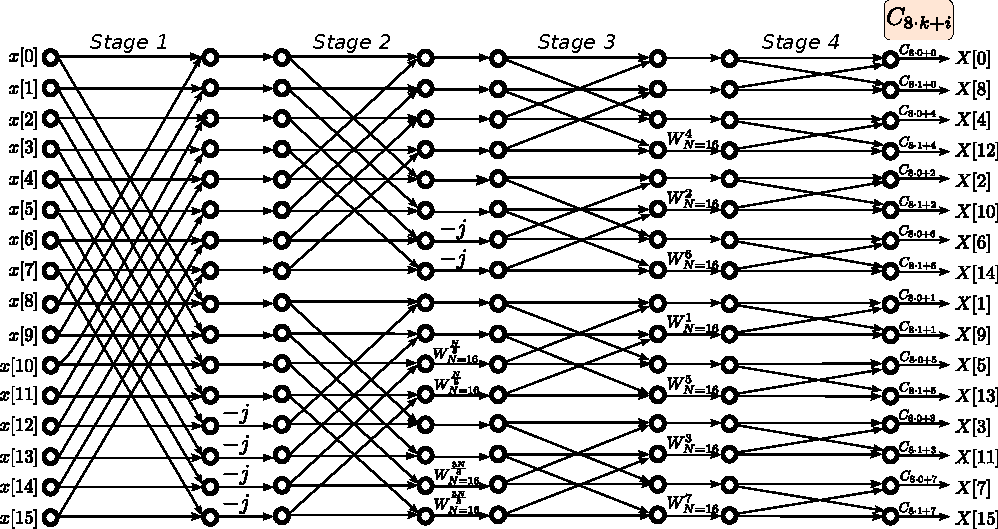
\includegraphics[width=0.75\paperwidth]{./image/16points_con.pdf}
    \caption{\footnotesize Flow graph of a radix-$2^3$ 16-point DIF DFT.}
    \end{figure}
\end{frame}
    
\begin{frame}
  	\frametitle{\textbf{The Radix-$2^3$ FFT  Algorithm}}
	\framesubtitle{\secname : \subsecname}
	

  \begin{block}{\centering \textbf{The Radix-$2^3$ FFT  Algorithm}}
    \vspace{-0.5cm}
    \begin{tabular}[c]{lr}
      %\hspace{-0.4cm}
      \begin{minipage}[t]{0.45\linewidth}
        \vspace{0.5cm}
        \begin{itemize} \justifying\footnotesize
        \item Applying (\ref{eqn:radix}) for the 128 point DFT and calculating each coefficient for $k=0,1,...,(128/8)-1$:
			\scalebox{1}{\parbox{0.45\linewidth}{    				
			\begin{equation*} 
				C_{8k+i} = \sum_{n=0}^{128/8-1} \{ \cdot \}
			\end{equation*}}}\\			         
         	We get a sequence in chain of butterflies with its corresponding rotation factor.
        \item The 128 point DFT goes through a processes that involve tree stages of butterflies to arrive finally to a set of eight DFT where each of one is a 16 point DFT.
        \end{itemize}
      \end{minipage}
      \hspace{0.3cm}
      \begin{minipage}[t]{0.45\linewidth}
        \vspace{0.5cm}
    \begin{figure}[h!] \centering
    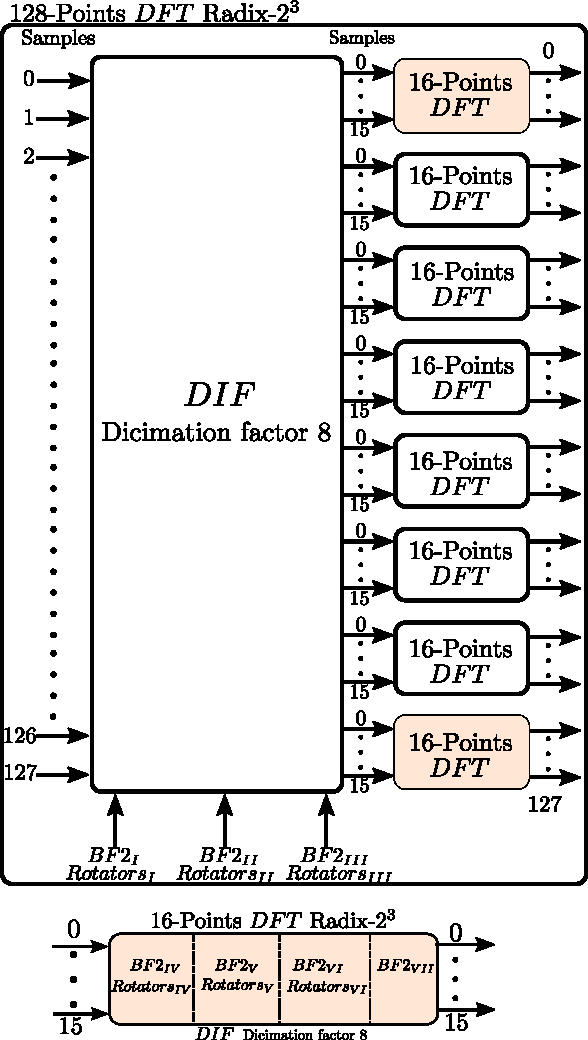
\includegraphics[height=0.6\paperheight]{./image/BloquesDft.pdf}
    \end{figure}
      \end{minipage}
    \end{tabular}
  \end{block}

\end{frame}




   % Radix 2^3 FFT Algorithm
\section{Design of FFT architecture via folding transformation}
\subsection{Parallel radix-$2^3$ 16-Points}
\begin{frame}
  \frametitle{\textbf{Table of Contents}}
  \begin{center}
    {\vspace{-1.5cm}\Large \textbf{Sección \thesection}\vspace{0.5cm}}
    \begin{beamercolorbox}[
      sep=8pt,center]{part title}
      \usebeamerfont{part title}
      \textbf{\insertsection}
    \end{beamercolorbox}
  \end{center}
\end{frame}


\begin{frame}
	\frametitle{\textbf{Design of FFT architecture via folding transformation}}
	\framesubtitle{\secname : \subsecname}
	
	\begin{block}{\centering \textbf{Folding Set}}
		\begin{itemize}\justifying\footnotesize
        	\item Is an ordered set of operations executed by the same functional unit.
        	\item Each folding set contains K entries, where K is called the folding factor.
        	\item The operation in the \textit{j}th position (where goes from 0 to K-1) is called the folding order.
       	\end{itemize}
	\end{block}

	\begin{block}{\centering \textbf{Folding Equations}}
		\begin{itemize}\justifying\footnotesize
			\item Consider an edge $e$ connecting the nodes \textit{U} and \textit{V} with $w(e)$ delays. 
			\item The executions of the \textit{l}th iteration of \textit{U} and \textit{V} are scheduled at the time units $Kl+u$ and $Kl+v$ respectively, where $u$ and $v$ are the folding orders of the nodes \textit{U} and \textit{V}.
			\item  The folding equation for the edge $e$ is:
			\begin{equation}\label{eqn:fold_equation}
				D_F(U \to V) = Kw(e)-P_U+v-u
			\end{equation}
			where $P_U$ is the number of pipeline stages in the node \textit{U}.
	    \end{itemize}
	\end{block}
\end{frame}


\begin{frame}
	\frametitle{\textbf{Design of FFT architecture via folding transformation}}
	\framesubtitle{\secname : \subsecname}
		\vspace{-0.5cm}
	    \begin{columns}[t,onlytextwidth]
	      \begin{column}{0.45\linewidth}
			\begin{block}{\centering \textbf{Folding equations without retiming/pipeline}}	      	
	        	\begin{itemize} \justifying\footnotesize
					\item Consider the folding sets:  \vfill
					\scalebox{0.65}{
					\label{eq:foldingset_16}		 
		 			\parbox{\linewidth}{ 
					\begin{align*}
						A&= \{ A0,A2,A4,A6 \}  & A'&= \{ A1,A3,A5,A7 \} \\
						B&=\{ B1,B3,B0,B2 \}   &B'&=\{ B5,B7,B4,B6 \} 	\\
						C&=\{ C2,C1,C3,C0 \}   &C'&=\{ C6,C5,C7,C4 \} 	\\ 
						D&=\{ D3,D0,D2,D1 \}   &D'&=\{ D7,D4,D6,D5 \}  
					\end{align*}}}
				
					\item For example: \vfill
					\scalebox{0.8}{
		 			\parbox{\linewidth}{ 				
					\begin{align*}
						D_F(D3\to B3)&= v - u \\
								 &= 0 - 1 \\  
								 &= -1
					\end{align*}}}
					\item The folding equations can be derived for all edges. \vfill
	      		\end{itemize}
			\end{block}	      
	      \end{column}
	      \begin{column}{0.50\linewidth}
	      	      \vspace{1cm}
			    \begin{figure}[h!] \centering
	    			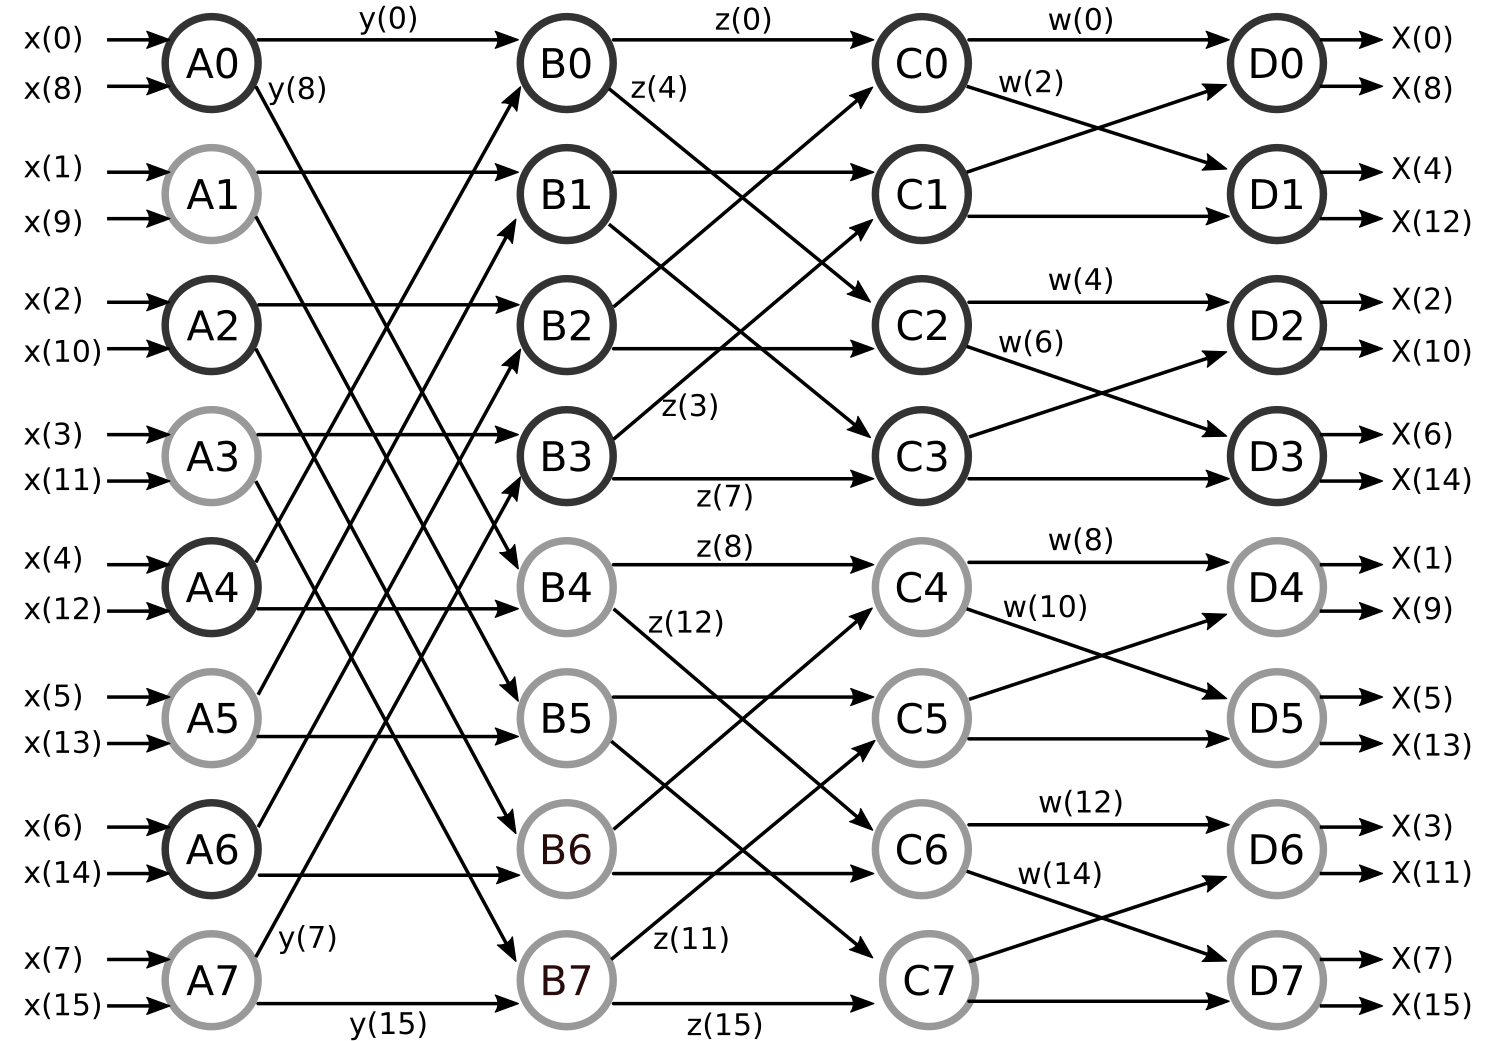
\includegraphics[width=0.45\paperwidth]{./image/16points_dfg.png}
	    			\caption{\footnotesize DFG of a radix-$2^3$ 16-point DIF DFT.}
	    		\end{figure}    
	      \end{column}
	    \end{columns}
\end{frame}




\begin{frame}
	\frametitle{\textbf{Design of FFT architecture via folding transformation}}
	\framesubtitle{\secname : \subsecname}
		\vspace{-0.5cm}
	    \begin{columns}[t,onlytextwidth]
	      \begin{column}{0.45\linewidth}
			\begin{block}{\centering \textbf{Folding equations with retimming/pipeline}}	      	
	        	\begin{itemize} \justifying\footnotesize
					\item For the folded system to be realizable, $D_F(U\to V)\geq0$ must hold for all the edges. \vfill
					\item For example: \vfill
						\scalebox{0.8}{
		 				\parbox{\linewidth}{ 				
						\begin{align*}
							D_F(D3\to B3)&= Kw(e) + v - u \\
								 &= 4(1) + 0 - 1 \\  
								 &= 3
						\end{align*}}}
						
					\item This result $D_F(U\to V)\geq0$ for all the edges.
					\item Applying the folding equations for all the edges, the number of registers required is 80. \vfill
	      		\end{itemize}
			\end{block}	      
	      \end{column}
	      \begin{column}{0.50\linewidth}
	      \vspace{1cm}
			    \begin{figure}[h!] \centering
	    			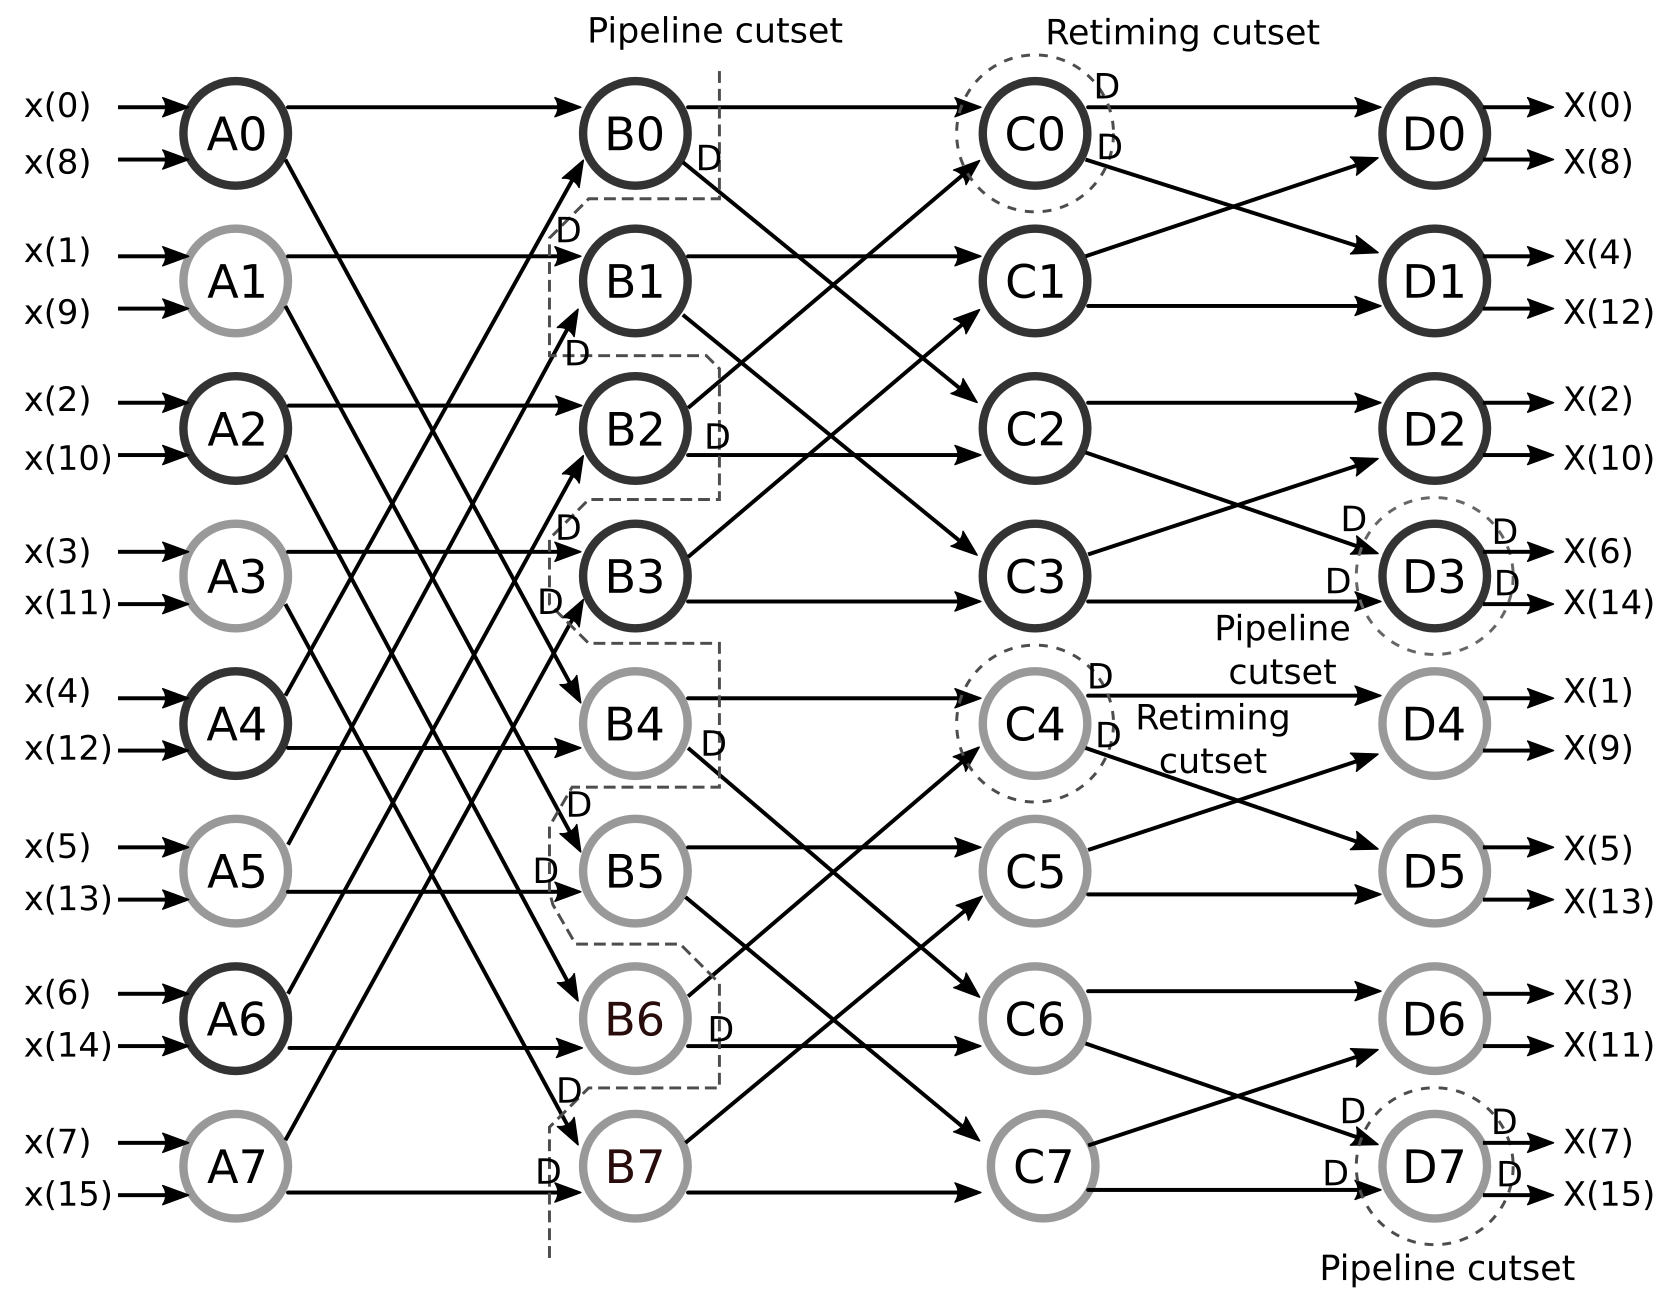
\includegraphics[width=0.45\paperwidth]{./image/16points_dfg_ret.png}
	    			\caption{\footnotesize DFG of a radix-$2^3$ 16-point DIF DFT applying pipeline and retiming.}
	    			\label{fig:16_point_ret}
	    		\end{figure}    
	      \end{column}
	    \end{columns}
\end{frame}

\begin{frame}
	\frametitle{\textbf{Design of FFT architecture via folding transformation}}
	\framesubtitle{\secname : \subsecname}
	\vspace{-0.5cm}
	 \begin{columns}[t,onlytextwidth]
	      \begin{column}{0.5\linewidth}
			\begin{block}{\centering \textbf{Lifetime analysis}}
				\begin{itemize}\justifying\footnotesize
					\item Is a procedure used to compute the minimun number of registers. \vfill
					\item For example, the variable $y_1$ be live during time units $n \in \{1,2,3,4\}$.
					\item The number of live variables $y_i$ during the time units $\{1,2,3,4,5\}$ is $\{4,8,8,8,4\}$. So the number of register for this stage is: \vfill
					\begin{equation*}
						max\{4,8,8,8,4\} = 8
					\end{equation*}
					\item The total number of registers is reduced from 80 to 20. \vfill
		       	\end{itemize}
			\end{block}
   		  \end{column}
   		  \begin{column}{0.5\linewidth}
   		  	 \vspace{-0.5cm}
   			\begin{figure}[h!] \centering
	    		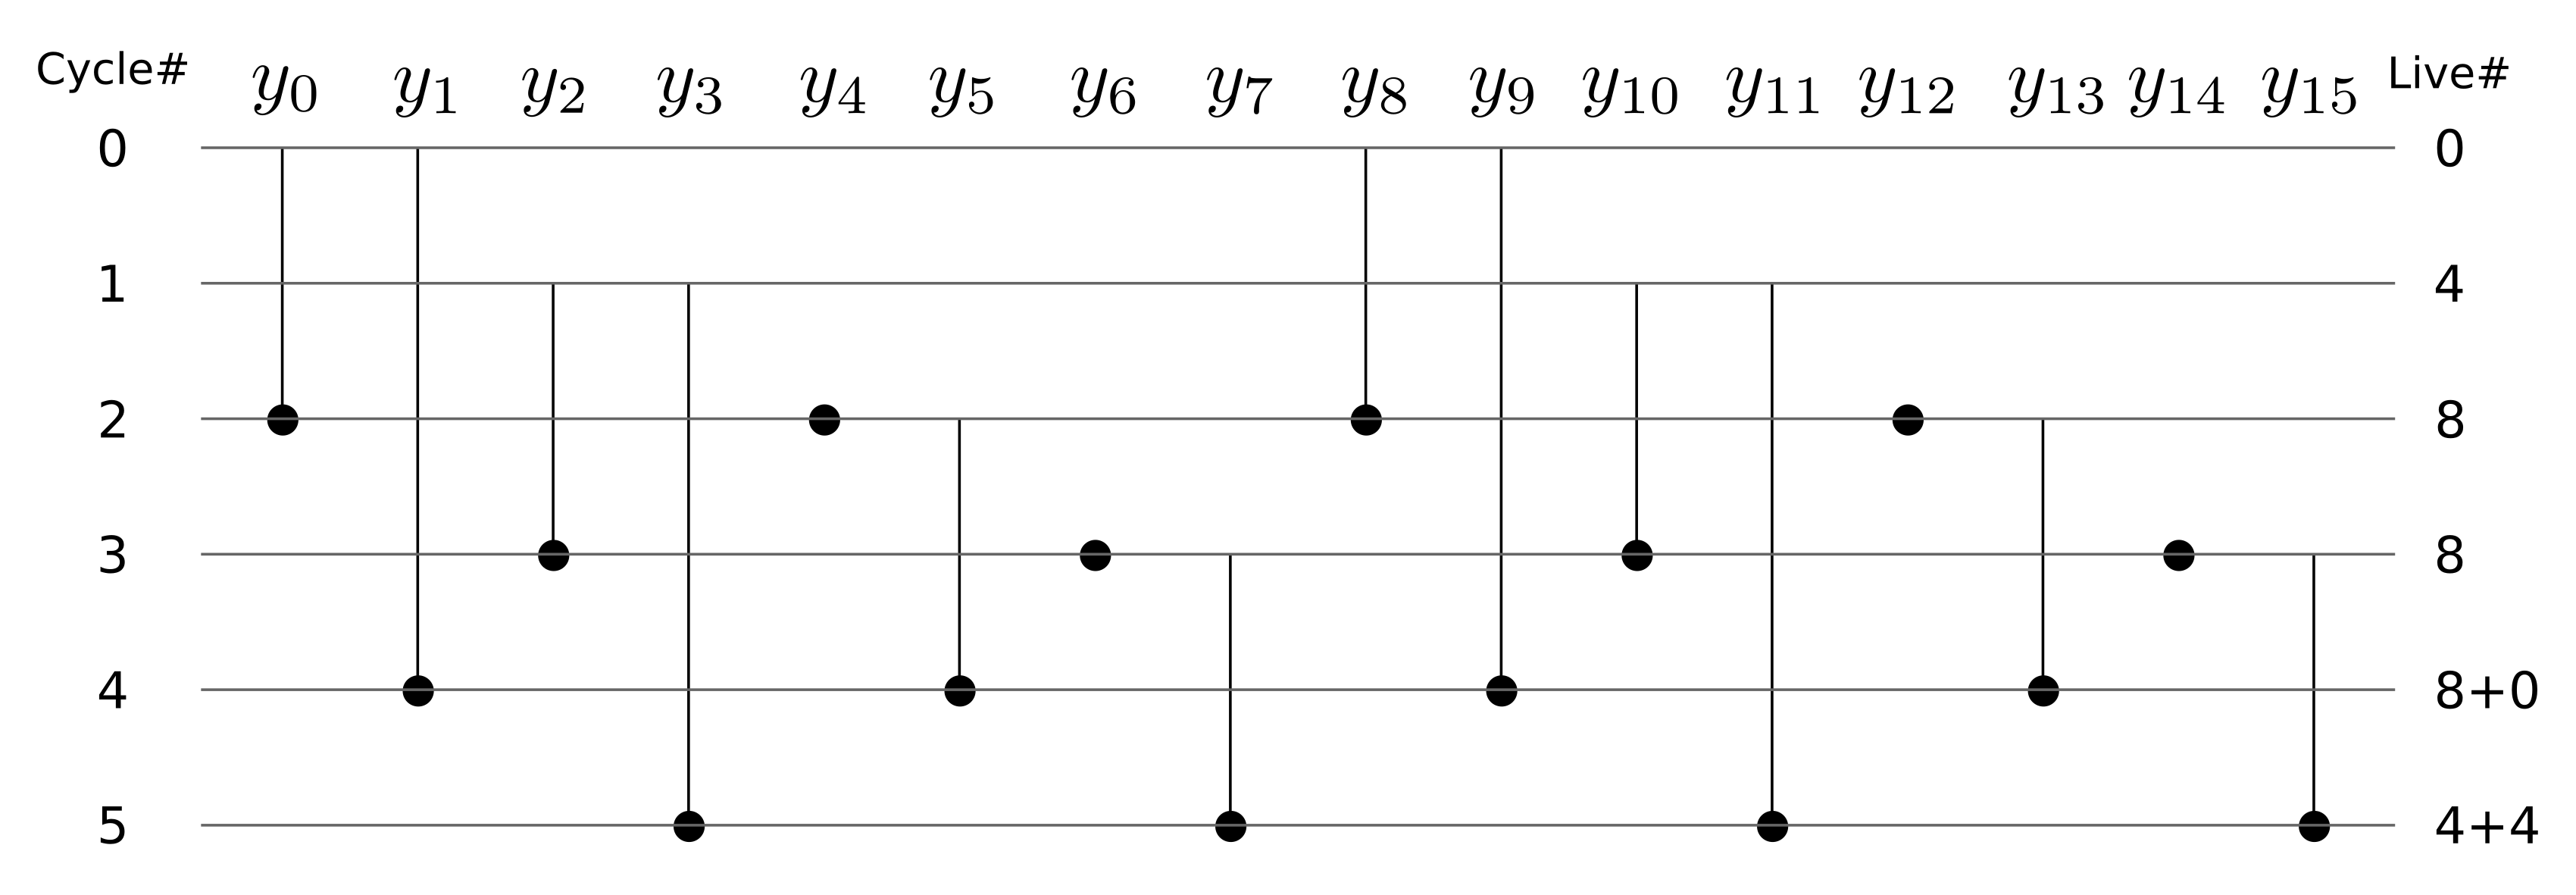
\includegraphics[width=0.40\paperwidth]{./image/life_chart_a.png}
	    		\caption{\footnotesize Lifetime chart for stage 1.}
	    	\end{figure}
	    	\vspace{-1cm}
	    	\begin{figure}[h!] \centering
	    		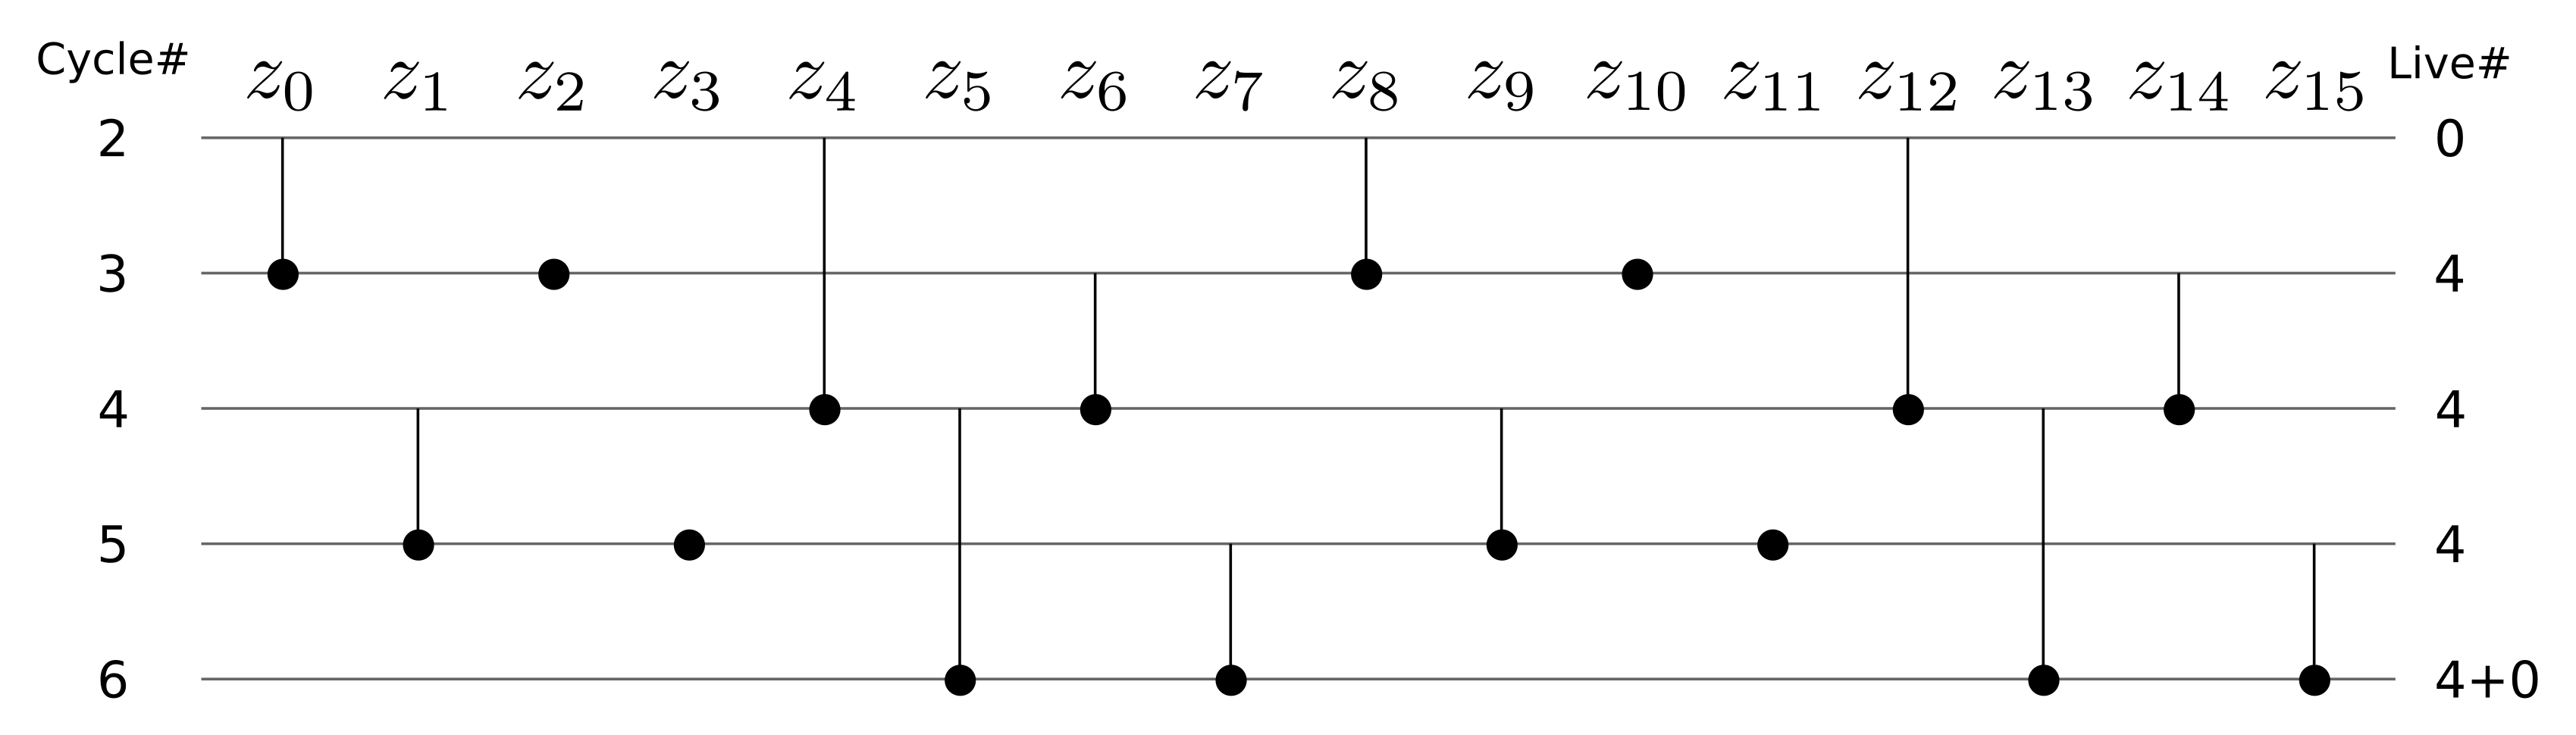
\includegraphics[width=0.40\paperwidth]{./image/life_chart_b.png}
	    		\caption{\footnotesize Lifetime chart for stage 2.}
	    	\end{figure}
			\vspace{-1cm}	    	
	    	\begin{figure}[h!] \centering
	    		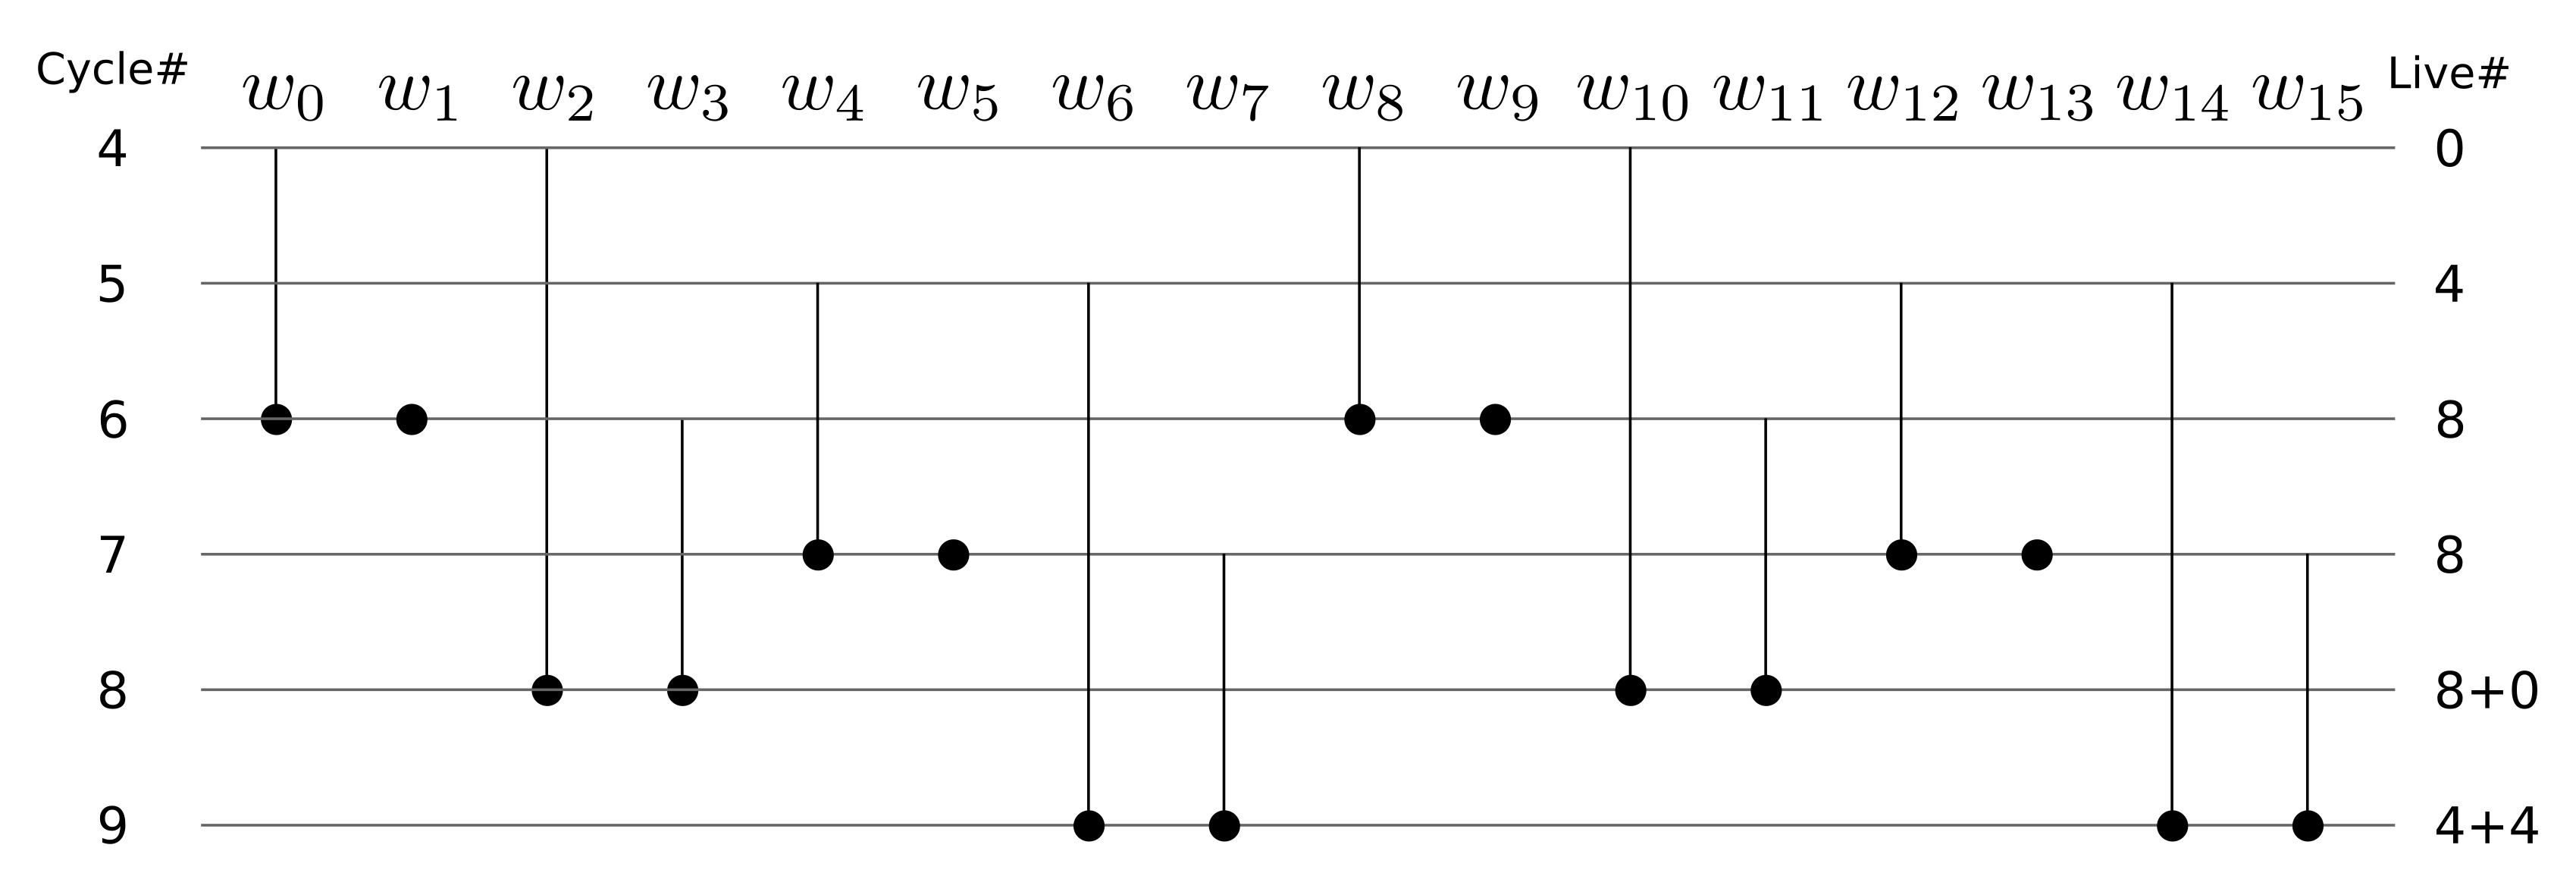
\includegraphics[width=0.40\paperwidth]{./image/life_chart_c.png}
	    		\caption{\footnotesize Lifetime chart for stage 3.}	    	
	    	\end{figure}  
   		\end{column}
	\end{columns}
\end{frame}

\begin{frame}
	\frametitle{\textbf{Design of FFT architecture via folding transformation}}
	\framesubtitle{\secname : \subsecname}
	\vspace{-0.5cm}
	 \begin{columns}[t,onlytextwidth]
	      \begin{column}{0.5\linewidth}
			\begin{block}{\centering \textbf{Forward Register Allcation}}
				\begin{itemize}\justifying\footnotesize
		        	\item This dictates how the variables are assigned to the minimum numbers of registers. \vfill
		        	\item If $R_i$ holds holds a variable in the current ctcle, then $R_{i+1}$ hold the same variable on the next cycle.
		       	\end{itemize}
			\end{block}
			\vspace{-0.3cm}
			\begin{figure}[h!] \centering
	    		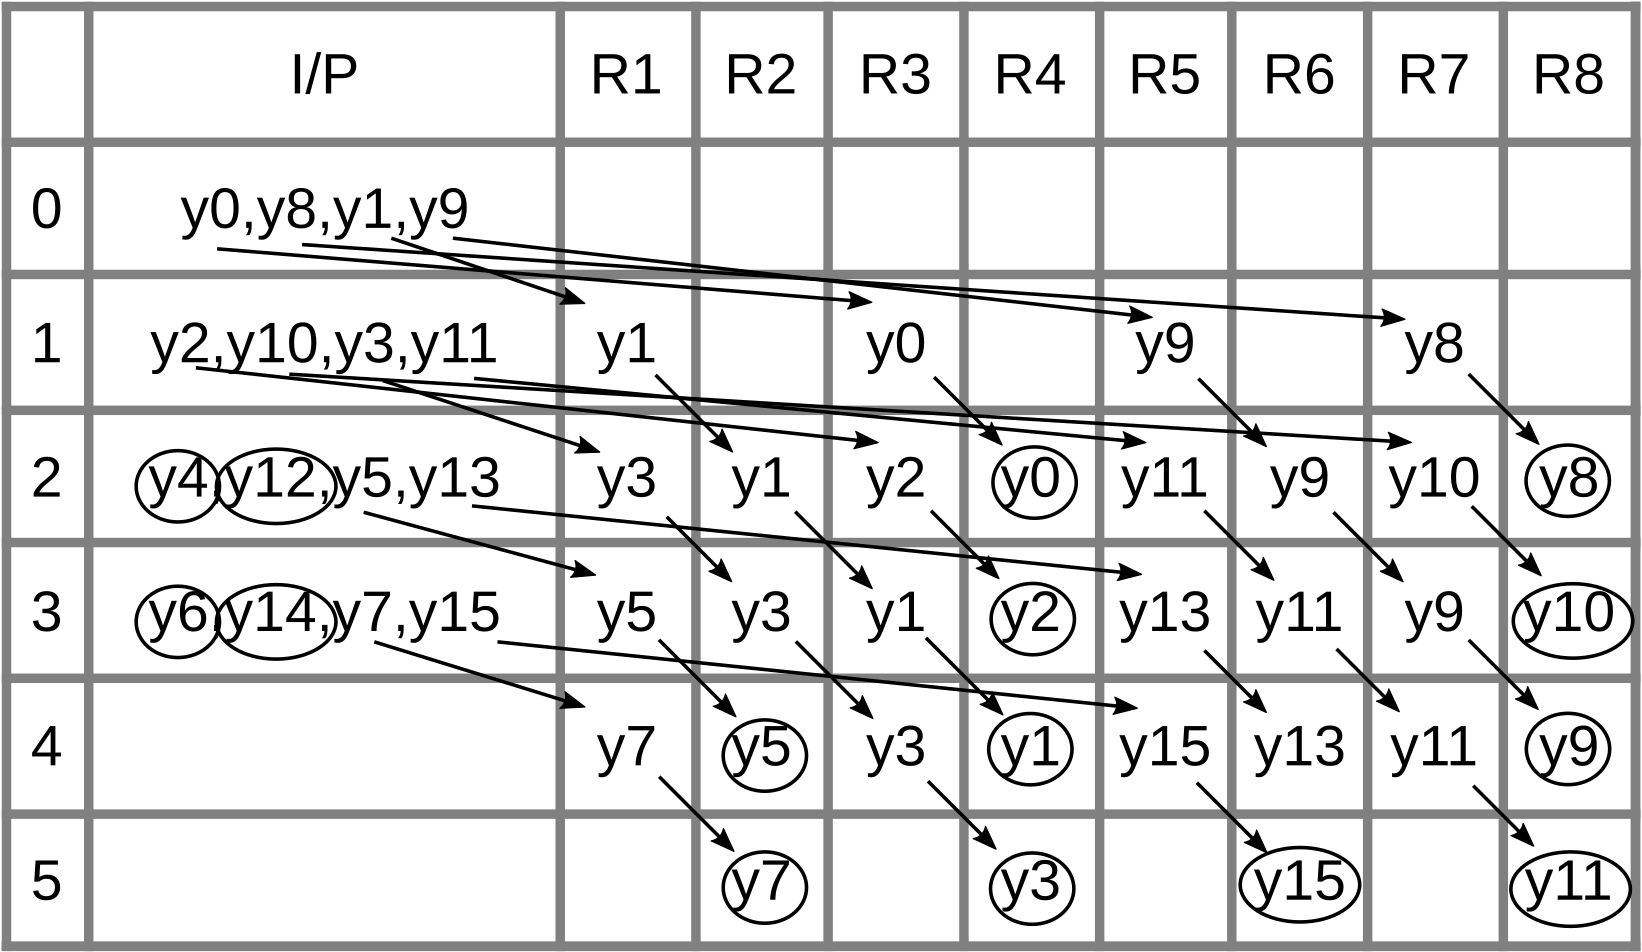
\includegraphics[height=0.30\paperheight]{./image/tab-life-a.png}
	    		\caption{\footnotesize Allocation table for stage 1.}
	    	\end{figure}
   		  \end{column}
   		  \begin{column}{0.45\linewidth}
   			\begin{figure}[h!] \centering
	    		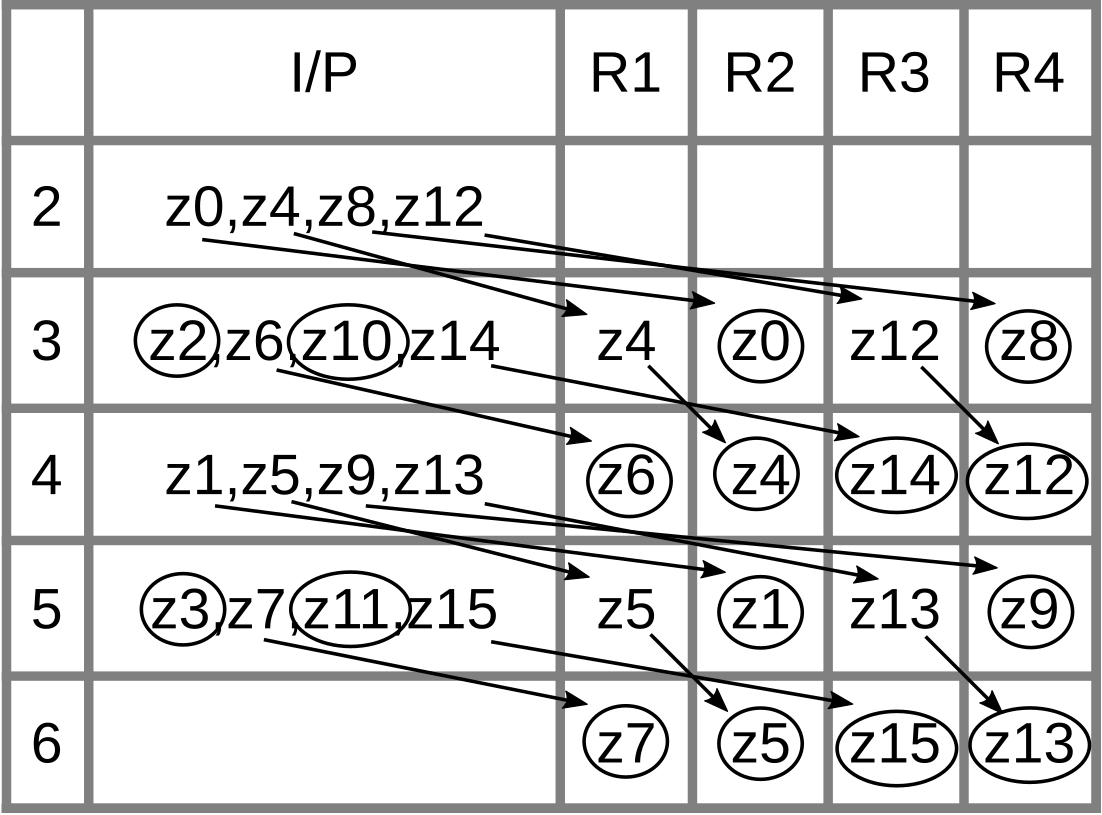
\includegraphics[height=0.25\paperheight]{./image/tab-life-b.png}
	    		\caption{\footnotesize Allocation table for stage 2.}
	    	\end{figure}
	    	\vspace{-0.75cm}
	    	\begin{figure}[h!] \centering
	    		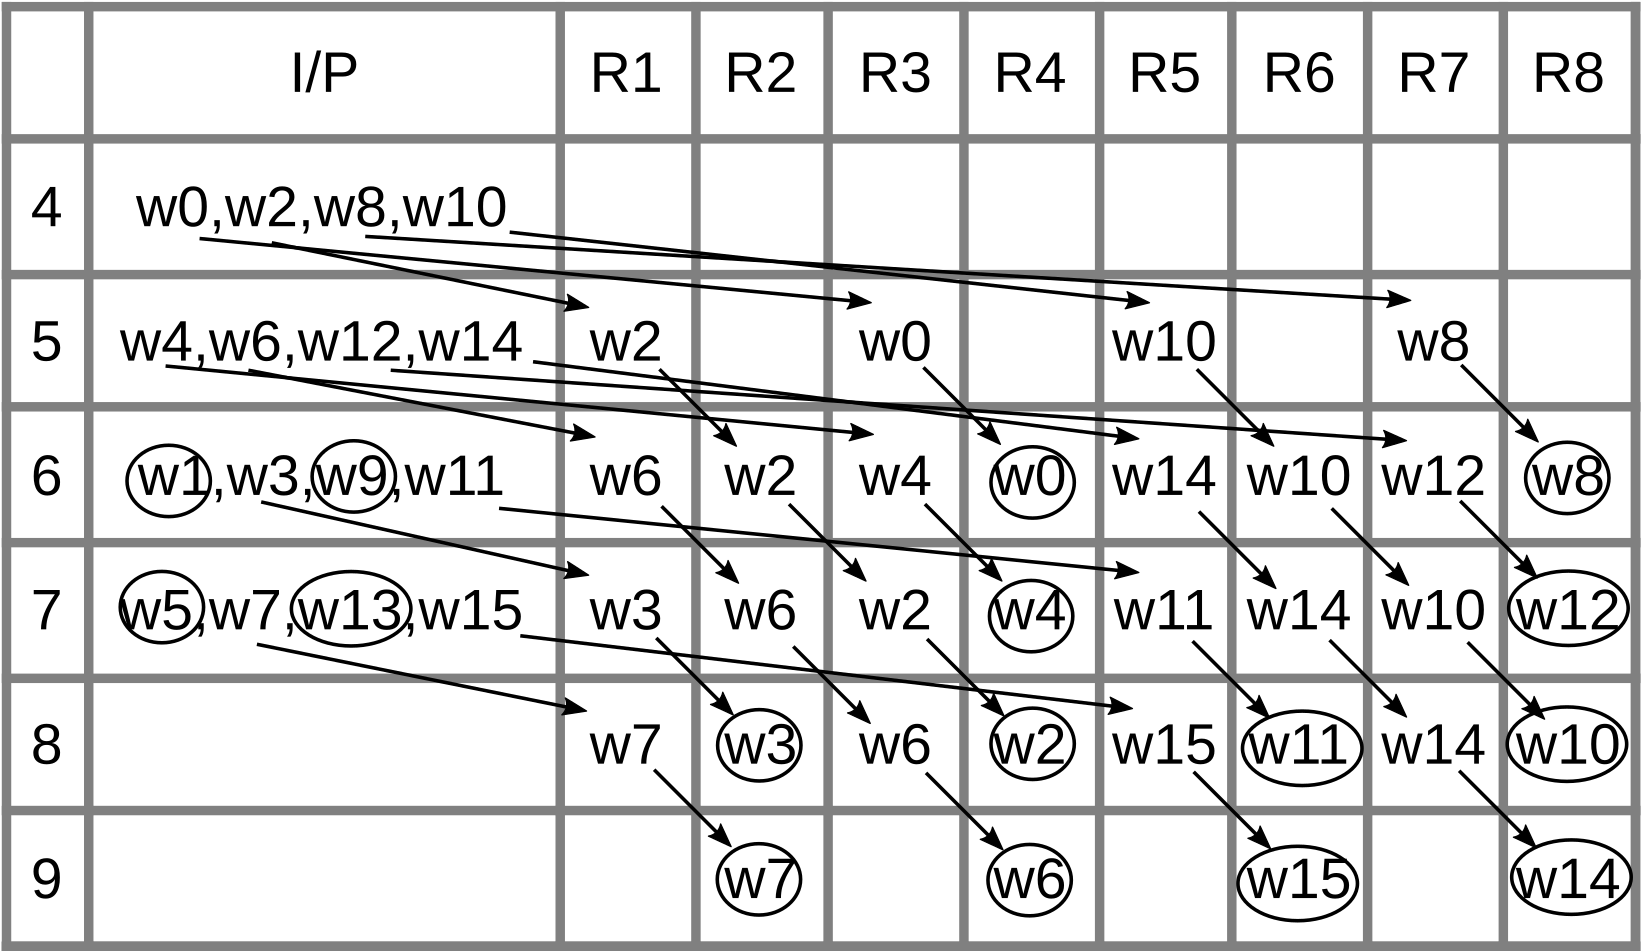
\includegraphics[height=0.30\paperheight]{./image/tab-life-c.png}
	    		\caption{\footnotesize Allocation table for stage 3.}
	    	\end{figure}  
   		\end{column}
	\end{columns}
\end{frame}

   % Design of FFT architecture via folding transformation
\section{Implementation}
\subsection{Parallel radix-$2^3$ 16-Points}
\begin{frame}
  \frametitle{\textbf{Table of Contents}}
  \begin{center}
    {\vspace{-1.5cm}\Large \textbf{Section \thesection}\vspace{0.5cm}}
    \begin{beamercolorbox}[
      sep=8pt,center]{part title}
      \usebeamerfont{part title}
      \textbf{\insertsection}
    \end{beamercolorbox}
  \end{center}
\end{frame}


\subsection{Floating and Fixed point Simulator}


\begin{frame}
	\frametitle{\textbf{Design of FFT architecture via folding transformation}}
	\framesubtitle{\secname : \subsecname}
	\begin{block}{\centering \textbf{Signal Quantization}}
		\begin{itemize}\justifying\footnotesize
        	\item The signals in each stage are quantized in order to obtain a high SQNR\footnote{Signal to Quantization Noise Ratio}($\approx 50\, dB$).
			\begin{equation*}%\label{eq:sqnr}
			SQNR_{dB} = 10log_{10} \bigg(  \frac{  Var\{Signal_{FloatPoint}\}  }{  Var\{Signal_{FloatPoint} - Signal_{FixedPoint}\}}  \bigg)
			\end{equation*}
			\item The quantization of the signals is:
			\begin{itemize}\justifying\footnotesize
				\item Input: $S(10,9)$, $SQNR \approx 57\,dB$.
				\item Twiddle factors: $S(11,9)$.
				\item Output: $S(22,15)$, $SQNR \approx 47\,dB$.				
			\end{itemize}			 
		\end{itemize}	
	\end{block}
\end{frame}



\begin{frame}
	\frametitle{\textbf{Design of FFT architecture via folding transformation}}
	\framesubtitle{\secname : \subsecname}
	\begin{block}{\centering \textbf{Testing signals}}
		\begin{itemize}\justifying\footnotesize
        	\item The input signal will be a mixture of two sinusoid signals with frecuencies  $f_1=100Hz$, $f_2=1000Hz$.
        	%\item This signal will be noramalized to the unity.
		\begin{align}\label{eq: inputSignal}
			x'[n] &= cos(2\pi f_1 n T_s) + cos(2\pi f_2 n T_s)  \\
			x[n] &= x'[n]/max\{x'[n]\} 						\nonumber
		\end{align}
		\end{itemize}	
	\end{block}
	\vspace{-0.75cm}
	\begin{columns}[t,onlytextwidth]
		\begin{column}{0.45\linewidth}
   			\begin{figure}[h!] \centering
	    		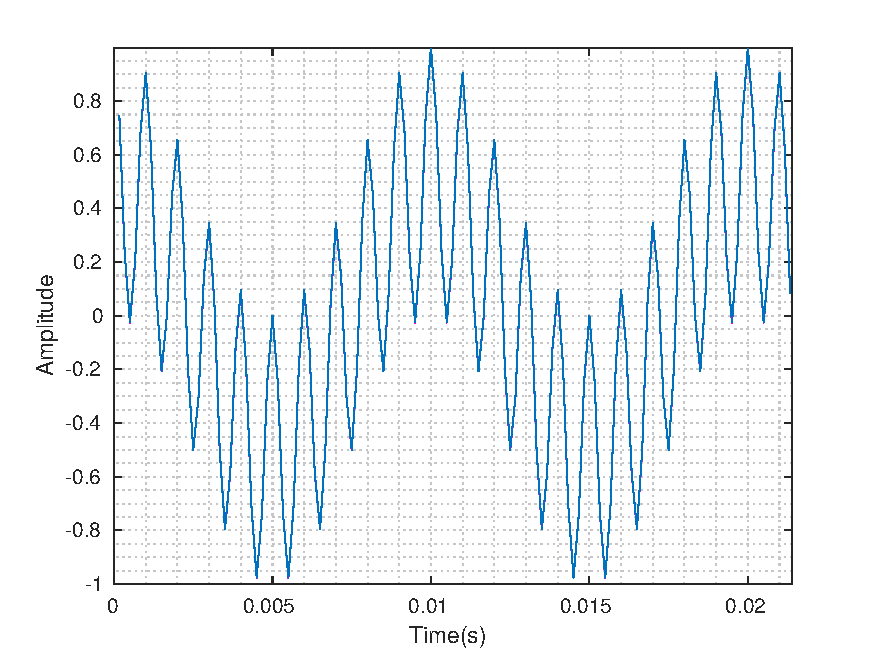
\includegraphics[height=0.35\paperheight]{./image/input_fx.pdf}
				\caption{\tiny Input signal $x[n]$ in time domain.}
	    	\end{figure}
	    \end{column}
	    \begin{column}{0.45\linewidth}
	    	\begin{figure}[h!] \centering
	    		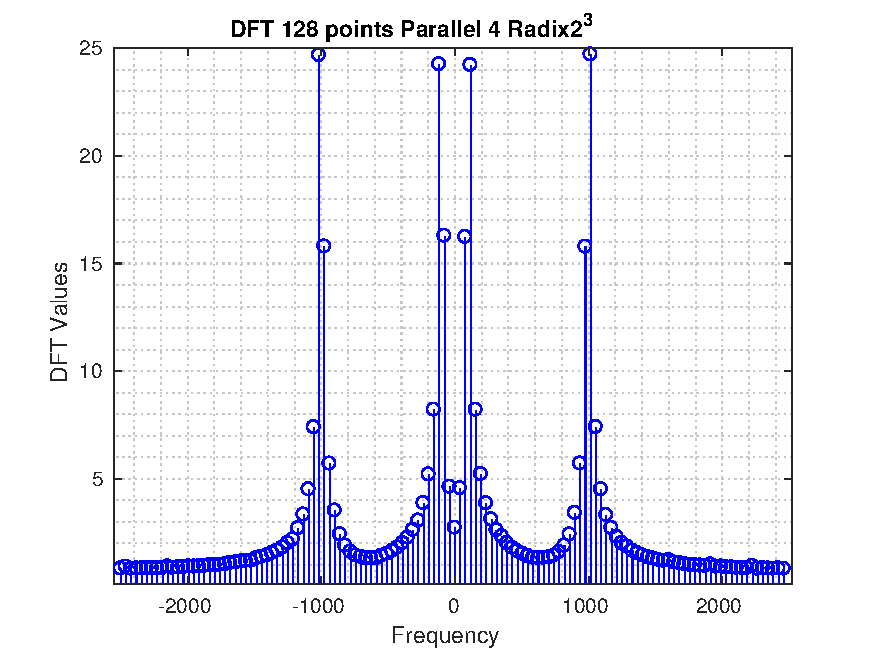
\includegraphics[height=0.35\paperheight]{./image/output_fx.pdf}
				\caption{\tiny Output samples, absolute value vs frequency $|X[k]|$.}
	    	\end{figure}  
   		\end{column}
	\end{columns}  
\end{frame}


\begin{frame}
	\frametitle{\textbf{Design of FFT architecture via folding transformation}}
	\framesubtitle{\secname : \subsecname}
	\begin{block}{\centering \textbf{Design Implementations}}
		\begin{itemize}\justifying\footnotesize
        	\item Design 1: 
        	\begin{itemize}\justifying\footnotesize
        		\item Quantitions blocks placed after the multiplers in each stage.
        		\item Multiplicators are not optimized.
			\end{itemize}        		 
        	\item Design 2:
			\begin{itemize}\justifying\footnotesize
				\item  A Pipeline cut-set is added after every quantization block.
			\end{itemize}				        	
        	\item Design 3:
        	\begin{itemize}\justifying\footnotesize
     			\item Implementation with Trival multiplicators for $-j$ factors. 
			\end{itemize}
        	\item Design 4:
        	\begin{itemize}\justifying\footnotesize
				\item A Pipeline cut-set is added inside of each butterfly block.				
				\item  Implementation of CSD multipliers.
			\end{itemize}
		\end{itemize}        	
	\end{block}
\end{frame}



\begin{frame}
	\frametitle{\textbf{Design of FFT architecture via folding transformation}}
	\framesubtitle{\secname : \subsecname}
	\vspace{-0.5cm}
		\begin{figure}[h!] \centering
		   	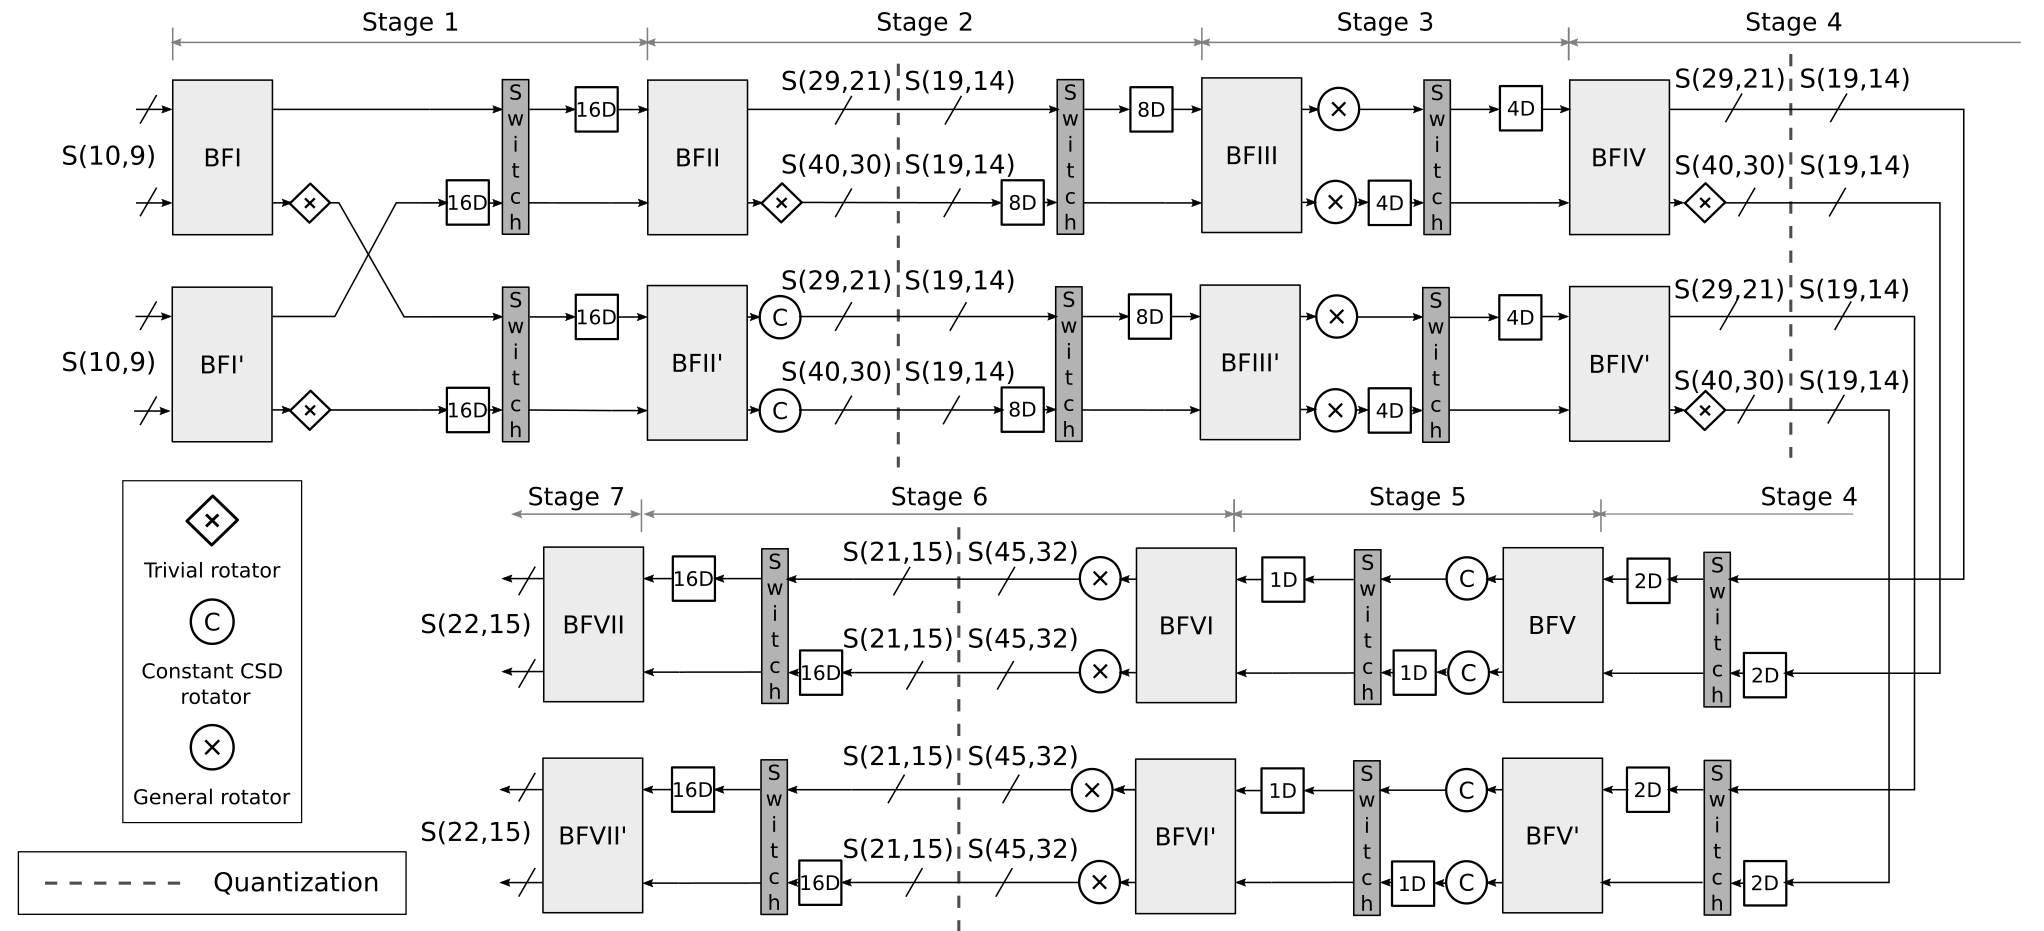
\includegraphics[width=0.95\paperwidth]{./image/folding-128-quant.png}
		   	\caption{ \tiny Folding architecture for radix-$2^3$  128 points FFT with quatization (Design 1).}
		\end{figure}  	
\end{frame}


\begin{frame}
	\frametitle{\textbf{Design of FFT architecture via folding transformation}}
	\framesubtitle{\secname : \subsecname}
	\vspace{-0.5cm}	
		\begin{figure}[h!] \centering
		   	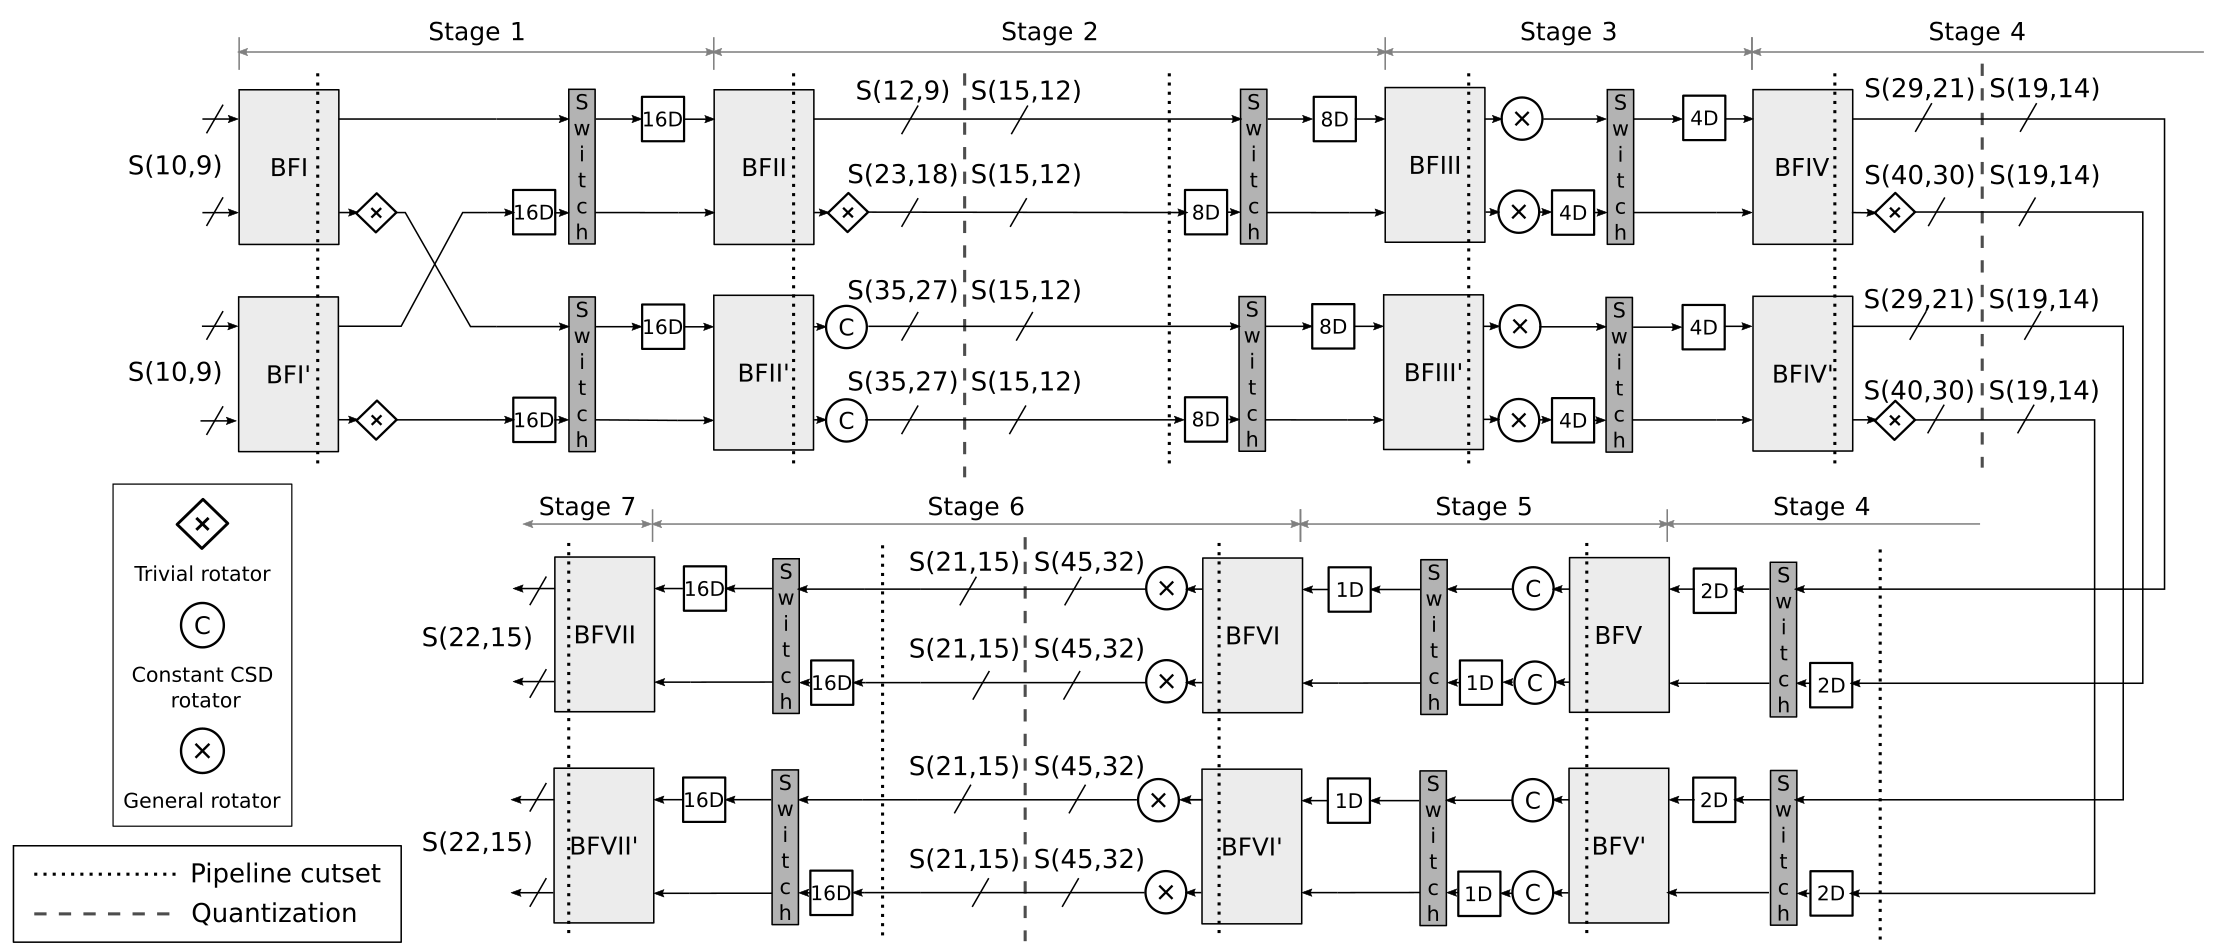
\includegraphics[width=0.95\paperwidth]{./image/folding-128-quant-pipe.png}
		   	\caption{ \tiny Folding architecture for radix-$2^3$ 128 points FFT with quantization and pipeline (Design 4).}
		\end{figure}  	
\end{frame}



\subsection{Results}

\begin{frame}
	\frametitle{\textbf{Design of FFT architecture via folding transformation}}
	\framesubtitle{\secname : \subsecname}
	\centering\textbf{Timing Report at 500MHz}
	\vspace{-0.75cm}
	\begin{columns}[t,onlytextwidth]
		\begin{column}{0.45\linewidth}
		   \begin{table}[t!]
			\centering%\raggedleft%\flushright 	
			\resizebox{0.6\linewidth}{!}{%			
			\begin{tabular}{@{}lr@{}}
				%\hline\hline
				Point 						& Path(ns)\\
				\hline\hline
				data arrival time   		& 5.60\\ 
				clock CLK (rise edge)  		& 2.00\\
				clock network delay (ideal) & 2.00\\
				library setup time			& 1.95\\
				\hline
				data required time			& 1.95\\
				data arrival time           & -5.60\\
				\hline
				slack (VIOLATED)            & -3.65\\	
				\hline
			\end{tabular}}
			\caption{\footnotesize Design instance 1.}			
			\end{table}
			%
			\vspace{-0.75cm}
			\begin{table}[t!]
			\centering%\raggedleft%\flushright 	
			\resizebox{0.6\linewidth}{!}{%
			\begin{tabular}{@{}lr@{}}
				%\hline\hline
				Point 						&Path(ns)\\
				\hline\hline
				data arrival time   		&2.76\\ 
				clock CLK (rise edge)  		&2.00\\
				clock network delay (ideal) &2.00\\
				library setup time			&1.95\\
				\hline
				data required time			&1.95\\
				data arrival time           &-2.76\\
				\hline
				slack (VIOLATED)            &-0.81\\	
				\hline
			\end{tabular}}
			\caption{\footnotesize Design instance 3.}
			\end{table}
   		\end{column}
   		%
		\begin{column}{0.45\linewidth}
			\begin{table}[t!]
			\centering%\raggedleft%\flushright 	
			\resizebox{0.6\linewidth}{!}{%			
				\begin{tabular}{@{}lr@{}}
				%\hline\hline
				Point 						&Path(ns)\\
				\hline\hline
				data arrival time   		&2.71\\ 
				clock CLK (rise edge)  		&2.00\\
				clock network delay (ideal) &2.00\\
				library setup time			&1.95\\
				\hline
				data required time			&1.95\\
				data arrival time           &-2.71\\
				\hline
				slack (VIOLATED)            &-0.76\\	
				\hline
			\end{tabular}}
			\caption{\footnotesize Design instance 2.}
			\end{table}
			\vspace{-0.75cm}
			\begin{table}[t!]
			\centering%\raggedleft%\flushright 	
			\resizebox{0.6\linewidth}{!}{%
			\begin{tabular}{@{}lr@{}}
				%\hline\hline
				Point 						& Path(ns)\\
				\hline\hline
				data arrival time   		&1.94\\ 
				clock CLK (rise edge)  		&2.00\\
				clock network delay (ideal) &2.00\\
				library setup time			&1.94\\
				\hline
				data required time			&1.94\\
				data arrival time           &-1.94\\
				\hline
				slack (MET)                 &0.00\\	
				\hline
			\end{tabular}}
			\caption{\footnotesize Design instance 4.}			
			\end{table}
   		\end{column}   		
	\end{columns}  
\end{frame}


\begin{frame}
	\frametitle{\textbf{Design of FFT architecture via folding transformation}}
	\framesubtitle{\secname : \subsecname}
	\centering\textbf{Area Report at 500MHz}
	\vspace{-1cm}
	\begin{columns}[t,onlytextwidth]
		\begin{column}{0.45\linewidth}
		   \begin{table}[t!]
			\centering%\raggedleft%\flushright 	
			\resizebox{0.65\linewidth}{!}{%			
				\begin{tabular}{@{}lr@{}}\\
				Logical Elements\\
				\hline\hline
				Number of ports               &1228\\
				Number of nets                &112376\\
				Number of cells               &102726\\
				Number of combinational cells &95310\\
				Number of sequential cells    &7404\\
				Number of macros/black boxes  &0\\
				Number of buf/inv             &27817\\
				\hline
				Combinational area            &291201.116637\\
				Buf/Inv area                  &44892.767764\\
				Noncombinational area         &58830.508095\\
				\hline
				Total cell area               &350031.624731\\	
				\hline
			\end{tabular}}
			\caption{\footnotesize Design instance 1.}			
			\end{table}
			%
			\vspace{-1.25cm}
			\begin{table}[t!]
			\centering%\raggedleft%\flushright 	
			\resizebox{0.65\linewidth}{!}{%			
			\begin{tabular}{@{}lr@{}}\\
				Logical Elements\\
				\hline\hline
				Number of ports                &1571\\
				Number of nets                 &94523\\
				Number of cells                &87311\\
				Number of combinational cells  &80220\\
				Number of sequential cells     &7076\\
				Number of macros/black boxes   &0\\
				Number of buf/inv              &23823\\
				\hline
				Combinational area             &233949.801414\\
				Buf/Inv area                   &36323.350042\\
				Noncombinational area          &56229.647552\\
				\hline
				Total cell area                &290179.448967\\	
				\hline
			\end{tabular}}
			\caption{\footnotesize Design instance 3.}
			\end{table}
   		\end{column}
   		%
		\begin{column}{0.45\linewidth}
			\begin{table}[t!]
			\centering%\raggedleft%\flushright 	
			\resizebox{0.65\linewidth}{!}{%			
			\begin{tabular}{@{}lr@{}}\\
				Logical Elements\\
				\hline\hline
				Number of ports                &1826\\
				Number of nets                 &114367\\
				Number of cells                &104198\\
				Number of combinational cells  &96271\\
				Number of sequential cells     &7912\\
				Number of macros/black boxes   &0\\
				Number of buf/inv              &26770\\
				\hline
				Combinational area             &294733.068172\\
				Buf/Inv area                   &41738.133324\\
				Noncombinational area          &62955.185703\\
				\hline
				Total cell area                &357688.253875\\	
				\hline
			\end{tabular}}
			\caption{\footnotesize Design instance 2.}
			\end{table}
			\vspace{-1.25cm}
			\begin{table}[t!]
			\centering%\raggedleft%\flushright 	
			\resizebox{0.65\linewidth}{!}{%			
			\begin{tabular}{@{}lr@{}}\\
				Logical Elements\\
				\hline\hline
				Number of ports                &2315\\
				Number of nets                 &75713\\
				Number of cells                &66284\\
				Number of combinational cells  &58017\\
				Number of sequential cells     &8240\\
				Number of macros/black boxes   &0\\
				Number of buf/inv              &14789\\
				\hline
				Combinational area             &195877.841872\\
				Buf/Inv area                   &24429.880240\\
				Noncombinational area          &64463.046570\\
				\hline
				Total cell area                &260340.888442\\	
				\hline
			\end{tabular}}
			\caption{\footnotesize Design instance 4.}			
			\end{table}
   		\end{column}   		
	\end{columns}  
\end{frame}

\begin{frame}
	\frametitle{\textbf{Design of FFT architecture via folding transformation}}
	\framesubtitle{\secname : \subsecname}
	\centering\textbf{Power Report at 500MHz}
	\vspace{-0.75cm}
	\begin{columns}[t,onlytextwidth]
		\begin{column}{0.45\linewidth}
			\begin{table}[t!]
			\centering%\raggedleft%\flushright 	
			\resizebox{\linewidth}{!}{%			
			\begin{tabular}{@{}lcccr@{}}\\
				Power Group		 &Internal 	&Switching 	&Leakage		&Total Power\\
				\hline\hline
				io pad           &0.0000    &0.0000     &0.0000    		&0.0000\\
				clock network    &34.8220   &603.2268   &1.4573e+06 	&639.6328\\
				register         &54.2228   &0.2699     &4.0540e+05 	&54.8980\\  
				sequential       &0.0000    &0.0000     &0.0000     	&0.0000\\  
				combinational    &0.2884    &0.7304     &1.5016e+04 	&1.0337\\ 
				\hline
				Total            &89.333mW  &604.227mW  &1.877e+06nW	&695.564mW\\	
				\hline
			\end{tabular}}
			\caption{\footnotesize Design instance 1.}			
			\end{table}
			\vspace{-1cm}
			\begin{table}[t!]
			\centering%\raggedleft%\flushright 	
			\resizebox{\linewidth}{!}{%
			\begin{tabular}{@{}lcccr@{}}\\
				Power Group		 &Internal 	&Switching 	&Leakage		&Total Power\\
				\hline\hline
				io pad           &0.0000    &0.0000     &0.0000    		&0.0000\\
				clock network    &24.2875   &583.5885   &1.0269e+06 	&608.9492\\
				register         &51.0349   &0.1728     &3.8748e+05 	&51.5952\\  
				sequential       &0.0000    &0.0000     &0.0000     	&0.0000\\  
				combinational    &0.9554    &1.1271     &1.8640e+05 	&2.2689\\ 
				\hline
				Total            &76.277mW  &584.888mW  &1.600e+06nW	&662.813mW\\	
				\hline
			\end{tabular}}
			\caption{\footnotesize Design instance 3.}								
			\end{table}
		\end{column}
		%
		\begin{column}{0.45\linewidth}
			\begin{table}[t!]
			\centering%\raggedleft%\flushright 	
			\resizebox{\linewidth}{!}{%			
			\begin{tabular}{@{}lcccr@{}}\\
				Power Group		 &Internal 	&Switching 	&Leakage		&Total Power\\
				\hline\hline
				io pad           &0.0000    &0.0000     &0.0000    		&0.0000\\
				clock network    &36.5175   &603.3234   &1.3702e+06 	&641.2228\\
				register         &57.8422   &0.2604     &4.3383e+05 	&58.5363\\  
				sequential       &0.0000    &0.0000     &0.0000     	&0.0000\\  
				combinational    &0.5748    &1.4180     &1.5702e+05 	&2.1498\\ 
				\hline
				Total            &94.934mW  &605.001mW  &1.961e+06nW	&701.908mW\\	
				\hline
			\end{tabular}}
			\caption{\footnotesize Design instance 2.}
			\end{table}
			\vspace{-1cm}   
			\begin{table}[t!]
			\centering%\raggedleft%\flushright 	
			\resizebox{\linewidth}{!}{%			
			\begin{tabular}{@{}lcccr@{}}\\
				Power Group		 &Internal 	&Switching 	&Leakage		&Total Power\\
				\hline\hline
				io pad           &0.0000    &0.0000     &0.0000    		&0.0000\\
				clock network    &18.1655   &581.6307   &7.8320e+05 	&600.6672\\
				register         &58.2275   &0.2873     &4.4422e+05 	&58.9591\\  
				sequential       &0.0000    &0.0000     &0.0000     	&0.0000\\  
				combinational    &0.7768    &0.9958     &1.5970e+05 	&1.9322\\ 
				\hline
				Total            &77.169mW  &582.913mW  &1.387e+06nW	&661.558mW\\	
				\hline
			\end{tabular}}
			\caption{\footnotesize Design instance 4.}			
			\end{table}
		\end{column}
	\end{columns}
\end{frame}
  % Implementación 
%\section{Conclusion}
\subsection{Parallel radix-$2^3$ 16-Points}
\begin{frame}
  \frametitle{\textbf{Table of Contents}}
  \begin{center}
    {\vspace{-1.5cm}\Large \textbf{Section \thesection}\vspace{0.5cm}}
    \begin{beamercolorbox}[
      sep=8pt,center]{part title}
      \usebeamerfont{part title}
      \textbf{\insertsection}
    \end{beamercolorbox}
  \end{center}
\end{frame}



\begin{frame}
	\frametitle{\textbf{Design of FFT architecture via folding transformation}}
	\framesubtitle{\secname : \subsecname}
	\begin{block}{\centering \textbf{}}
		\begin{itemize}\justifying\footnotesize
        	\item 	 
		\end{itemize}	
	\end{block}
\end{frame}  % Conculsion




%
%\section{Bibliografía}
%\begin{frame}%[t,allowframebreaks]
%  \frametitle{Bibliografía}
%  % \vspace{-0.7cm}
%  \tiny
%  %\bibliographystyle{./IEEEtranBST/IEEEtran}
%  \bibliographystyle{ieeetr}
%  \bibliography{./biblio.bib}
%\end{frame}


\begin{frame}
  \frametitle{\textbf{Questions}}
   \begin{center}
     {\Huge \textbf{Thanks!}\\}
    \end{center}
\end{frame}

\end{document}
